\documentclass[prd,twocolumn,superscriptaddress,floatfix,amsmath,amssymb,amsfonts,nofootinbib]{revtex4-2}
%Change to prd to get emails in the right place, for ar\bar{x}iv.

\usepackage{float} 
\usepackage{comment}
\usepackage[normalem]{ulem}
\usepackage[english]{babel}
\usepackage{graphicx}% Include figure files
\usepackage{dcolumn}% Align table columns on decimal point
\usepackage{bm}% bold math
\usepackage{blindtext}
\usepackage{verbatim}
\usepackage{mathrsfs}
\usepackage{musicography}
\usepackage{amsmath}
\usepackage{dsfont}
\usepackage{cancel}
\usepackage{physics}
\usepackage{epstopdf}
\usepackage{mathtools}
\usepackage{color}
\usepackage[usenames,dvipsnames]{pstricks}
\usepackage{epsfig}
\usepackage{pst-grad} % For gradients
\usepackage{pst-plot} % For axes
\usepackage{hyperref}
\usepackage{verbatim}
\usepackage{afterpage}
\usepackage{arydshln}
\hypersetup{
    colorlinks=true,
    linkcolor=blue,
    filecolor=magenta,      
    urlcolor=cyan,
}

\usepackage{tikz}
\usetikzlibrary{quantikz}

\newcommand{\ii}{\mathrm{i}}
\setlength{\unitlength}{1cm}
\renewcommand{\d}{\mathrm{d}}
%\renewcommand{\vec}{\text{vec}}
\newcommand{\be}{\begin{equation}}
\newcommand{\bel}[1]{\begin{equation}\label{#1}}
\newcommand{\ee}{\end{equation}}
\newcommand{\tcb}{\textcolor{blue}} 
\newcommand{\tcr}{\textcolor{red}}
\newcommand{\tcg}{\textcolor{green}}

\newcommand{\mf}{\mathsf}%\mathsf is too long
\newcommand{\modify}[1]{\textcolor{black}{#1}}
\newcommand{\END}{\color{black}}%
\newcommand{\funnyx}{{\scriptstyle{\bm{\mathfrak{X}}}}}
\newcommand{\barsf}[1]{\bar{\mathsf{#1}}}
\newcommand{\timelike}{\musNatural}
\newcommand{\lightlike}{\rotatebox[origin=c]{135}{\musNatural}}
\newcommand{\spacelike}{\rotatebox[origin=c]{90}{\musNatural}}
\newcommand{\Dan}[1]{{\color{red}\bf [Dan: #1]}}

\begin{document}

\title{The Pragmatic QFT Measurement Problem\\ and the need for a Heisenberg-like Cut in QFT}

\author{Daniel Grimmer}
\email{daniel.grimmer@philosophy.ox.ac.uk}
\affiliation{Reuben College, University of Oxford, Oxford, OX2 6HW United Kingdom}
\affiliation{Faculty of Philosophy, University of Oxford, Oxford, OX2 6GG United Kingdom}
\affiliation{Barrio RQI, Waterloo, Ontario N2L 3G1, Canada}

\begin{abstract}
Despite quantum theory's remarkable success at predicting the (statistical) results of experiments, many philosophers worry that it nonetheless lacks some crucial connection between theory and experiment. Such worries are at the root of the Quantum Measurement Problem. We can identify two kinds of worries: 1) pragmatic: it's unclear how to model our experiments to extract theoretical predictions, and 2) realist: there is no realist narrative for the experiment underlying these theoretical predictions. While both worries deserve attention, the pragmatic worries have far worse consequences if left unanswered. Moreover, as I will argue, upon reflection, a satisfactory explanation of almost all of quantum theory's experimental successes unavoidably involves modeling quantum fields at some point. Thus, without a pragmatic theory-to-experiment link for QFT, we are at risk of losing any right to claim evidential support for large parts of quantum theory. Hence, I focus on the \textit{Pragmatic QFT Measurement Problem}.

But, what makes modeling measurements in QFT so hard? As I will discuss, attempts to naively transplant our non-relativistic quantum measurement theory into QFT are deeply unphysical and unsatisfying. Thus we need a new (or at least refined) measurement theory for QFT. However, as I will argue, aiming too directly at a new measurement theory is an incautious way to proceed and is apt to lead us astray. This paper proposes an alternate way forward: We ought to first better understand how our non-relativistic quantum measurement theory is rooted in notions of measurement chains and Heisenberg cuts. Then we ought to generalize these notions and transplant them into QFT. Such a transplant is carried out in this paper. My analysis suggests the need for a pragmatic \textit{QFT-cut} analogous to the need for a pragmatic Heisenberg cut in non-relativistic contexts.
\end{abstract}

\maketitle
\section{Introduction: A Quantum Measurement Problem}\label{Introduction}
It is uncontestable that quantum theory has been remarkably successful at predicting the (statistical) results of a wide range of experiments. However, despite its many predictive successes, many philosophers are nonetheless worried that quantum theory lacks some crucial connection between theory and experiment. Various dissatisfactions with various theory-to-experiment disconnects each deserve the title\footnote{This situation is rather like the mis-advertised efforts to ``find \textit{the} cure for cancer''. There are many types of cancer each of which will need their own cure. Moreover, even considering a single type of cancer, it may be cured in several ways.} ``A Quantum Measurement Problem'': How are we to understand/model the measurement of quantum systems?
    
In order to differentiate the various kinds of dissatisfactions from each other, it's perhaps best to start from a telling of quantum theory which (hopefully nearly) every philosopher is dissatisfied with. I have in mind the parts of quantum theory which students are urged to focus on after they are told to ``Shut up, and calculate!''. Let us call this \textit{the sophomore's quantum theory}. Students are here taught to model quantum experiments as follows: Given some initial conditions we apply the given unitary evolution and then the given projective measurement. This computation unambiguously gives a statistical prediction of the experiment's outcome via Born's rule. (A sophisticated sophomore may also learn about non-projective measurements, selective measurements and non-selective measurements as well as post-measurement state updates via L\"uders rule.) Many philosophers are dissatisfied with the sophomore's quantum theory and claim that it lacks the right kind of connection between theory and experiment.

At this point I would like to distinguish between two types of worries surrounding quantum measurement: pragmatic worries and realist worries. Pragmatic worries are aimed at clarifying how exactly these statistical predictions are to be pulled out of the theory. Specifically, how should the measurement process be \textit{modeled}? By contrast, realist worries are aimed at establishing a realist narrative for the measurement process. How could the world be such that our experiments have these statistics? What explains the different definite outcomes I see in each seemingly identical run of my experiment? How should the quantum measurement process be \textit{understood}?

The sophomore's quantum theory fails on both fronts. Its realist failures are well known, but its pragmatic failures deserve some further comment. The sophomore's quantum theory does not, in fact, give us unambiguous statistical predictions for the experiment's outcomes. While it is true that statistical predictions can be unambiguously associated with initial states, unitaries and projectors, $p(\text{out}\vert\,\hat{U},\text{in})=\vert\!\bra{\text{out}}\hat{U}\ket{\text{in}}\!\vert^2$, these themselves have not yet been suitably connected with our real-life experimental setups. Specifically, the sophomore has no answer to the question\footnote{The sophomore's question will be answered in Sec.~\ref{ChainsAndCuts3}. One answer involves decoherence theory and the Born rule. It should be noted, however, that contrary to popular belief, there may be other methods of extracting predictions from quantum theory in a principled way.}: ``In modeling this piece of lab equipment, exactly which projectors am I supposed to use and when?'' There may be a ready-answer to this question pre-written on the sophomore's  problem sheets, but show them a foreign piece of lab equipment and watch them falter. Often the sophomore may intuitively guess which projector to use and when. Moreover, their guesses may consistently give accurate-enough predictions, but ultimately they are nothing more than just that, guesses.

Of these two types of failings, which has worse consequences if neglected? While both deserve attention, I argue the pragmatic worries are by far more important since if unanswered their consequences are far more severe. While it is at least debatable whether or we need to find a realist narrative underlying quantum theory~\cite{sep-qt-issues}, it is not debatable that quantum theory (indeed, any physical theory) must provide us with a robust account\footnote{Above, I complained that the sophomore's quantum theory doesn't give us unambiguous predictions. However, on reflection, demanding complete unambiguity is asking too much. As I will discuss later, even for non-relativistic quantum theory it is necessary to make approximations when extracting concrete experimental predictions from our theory. Often we will have freedom (and hence ambiguity) regarding what kind of approximations we should make and where to make them. There is nothing wrong with this so long as the consequences of these choices are well understood and controllable. Indeed, when attempting to explain our experimental data, the goal is not to give definite unambiguous predictions but rather to give predictions which are within the experiment's error bars.} of how predictions can and should be made from it (something better than intuitive guessing, even if our guesses are often right). It is exactly this pragmatic link to real-life experimental practice which grants our physical theories evidential support, and arguably their physicality~\cite{Curiel} as well. Without a clear understanding of this pragmatic connection between theory and experiment, we are at risk of losing any right to claim evidential support (or worse physicality) for our theory. As interesting as the realist's worries are, I rather say: let us first work on bringing home the spoils of experimental success, then we can worry about what it all means later, once we have better footing.

As discussed above, the sophomore's quantum theory fails on both the pragmatic and realist fronts, but how do more sophisticated tellings of quantum theory fair? I will argue (in Sec. \ref{ChainsAndCuts}) that for non-relativistic quantum theory these pragmatic worries have been more-or-less satisfactorily handled in terms of measurement chains and pragmatic Heisenberg cuts. Consequently, in the non-relativistic case almost all attention has shifted onto the realist's worries. And rightly so. This so much so that for non-relativistic quantum theory the quantum measurement problem has become synonymous with such realist worries.

However, as I will argue (in Sec. \ref{WhatBlocksTheirWay}), these pragmatic worries have not yet been adequately dealt with for quantum field theory\footnote{Throughout this paper, unless specified otherwise, QFT refers to relativistic quantum field theory (as opposed to non-relativistic quantum field theory). Similarly, by non-relativistic quantum theory I mean, unless specified otherwise, first quantized quantum theories (e.g., not non-relativistic quantum field theory).} (QFT), with severe consequences; Without this crucial theory-to-experiment link we are at risk of losing any right to claim any evidential support (or worse physicality) for quantum field theory. Given the severity of this situation, the focus of this paper is exclusively on such pragmatic worries in the context of quantum field theory. That is, my focus is on \textit{The Pragmatic QFT Measurement Problem}

My suggestion that we first work on ``bringing home the spoils of experimental success'' raises the following questions: for quantum theory generally, where were these metaphorical spoils won and what currently blocks their way home? In Sec.~\ref{WhereTheSpoilsWereWon}, I will discuss where the evidential spoils lie so-to-speak. I will argue (paralleling Wallace~\cite{WallaceBlueSkyTalk,WallaceBlueSkyPaper}) for the following perhaps surprising claim; Explaining all but maybe a small corner of quantum theory's experimental successes unavoidably involves modeling quantum fields. (Importantly, this is for basic conceptual reasons; I am not here demanding hyper-accuracy.) Thus, if we cannot establish an adequate pragmatic link between QFT and experimental practice then not only quantum field theory but nearly the whole of quantum theory is at risk of losing its evidential support. While the argument in Sec.~\ref{WhereTheSpoilsWereWon} is not essential for the philosophical points made in the rest of the paper, it substantially raises the stakes.

Given that the route home for most of our experimental spoils runs through quantum field theory, our next question becomes: Why is it (at least currently) so hard to properly model measurements involving quantum fields? Sec.~\ref{WhatBlocksTheirWay} will answer this question.  As a growing portion of the physics community is now becoming aware~\cite{pologomez2021detectorbased,Jubb2022,BorstenJubbKells,fewster1,fewster2,fewster3,Anastopoulos2022,Sorkin,TaleOfTwo,Ruep2021,JoseMariaEdu,Redhead1995,Dowker,Dowker2,borsten,alvaro,Adam}, the hand-wavy measurement models for QFT described in most textbooks on quantum field theory, quantum optics and particle physics are deeply unphysical and unsatisfying. Why is this so?

It is often said~\cite{pologomez2021detectorbased,Jubb2022,BorstenJubbKells,fewster1,fewster2,fewster3,Anastopoulos2022,Sorkin,TaleOfTwo,Ruep2021,JoseMariaEdu,Sorkin,Redhead1995,Dowker,Dowker2,borsten,alvaro,Adam} that the unphysical nature of these textbook measurement models can be traced to certain non-trivial mathematical differences between QFT and non-relativistic quantum theory (e.g., new causal and algebraic structures at play). These differences disallow us from directly transplanting our non-relativistic quantum measurement theory into QFT. Proceeding naively leads us to make mathematical blunders which either violate the central `commandments' of relativity (covariance, causality, and locality)\cite{Sorkin,Redhead1995,Dowker,Dowker2,borsten,alvaro,Adam} or otherwise disrespect the QFT's local algebraic structure. For these reasons, it has been argued we need a new (or at least refined) measurement theory for quantum field theory, see for instance~\cite{pologomez2021detectorbased,Jubb2022,fewster2}.

While all of this is true, I argue that laying the blame on these technical issues belies a deeper methodological issue. Specifically, I will argue in Sec.~\ref{WhatBlocksTheirWay} that, even when one avoids all such mathematical blunders, other critical symptoms of a deeper methodological issue still remain. In fact, this root methodological issue is the same issue that plagues the sophomore's quantum theory: failure to give concrete models of our measurement processes, opting instead for simply guessing the right projector.

In this paper, I propose and carry out an alternate way forward: First, we ought to understand that our non-relativistic quantum measurement theory has its roots in discussions of measurement chains and Heisenberg cuts (Sec.~\ref{ChainsAndCuts}). Then, we ought to generalize these notions and transplant them into QFT (Sec.~\ref{GenChainsAndCuts} and Appendix~\ref{Appendix1}). Finally, by reviewing the current state of the art in the physics literature, we can then see what measurement theory, if any, we currently have for QFT (Sec.~\ref{StateOfTheArt}).

My analysis will reveal that analogous to the need for a pragmatic Heisenberg cut when modeling quantum experiments, we need to take a pragmatic Heisenberg-like cut when modeling quantum field theoretic experiments. I will call\footnote{This concept was first introduced in \cite{TaleOfTwo} under the name \textit{relativistic cut}. However, after publication we realized this name is apt to cause confusion. For reasons I will discuss in Sec.~\ref{GenChainsAndCuts} I believe the name \textit{QFT-cut} to be more appropriate.} this a \textit{QFT-cut}. As I will discuss, for either pragmatic Heisenberg cuts or QFT-cuts there are many kinds of cuts available to us, each of which can help us extract predictions from our theory in a principled way. As I will discuss, ultimately, the notions of measurement chains and cuts provide us with, for each experiment under consideration, a road map to guide us in modeling its specific measurement processes. That is, an understanding of measurement chains and cuts in the context of QFT gives us a case-by-case measurement framework for quantum fields. However, in order to achieve a more wide-scoping measurement theory for QFT we need to identify some way of crossing the FT-cut which can be applied to our experimental setups near-universally. As I will discuss, our current best tool for getting a wide-scoping measurement theory for QFT is the Unruh-DeWitt detector model~\cite{Unruh1976,BLHu2007, Brown2013, Hotta2020, Zeromode,TaleOfTwo,Adam,Valentini1991, Reznik2003, Pozas-Kerstjens:2015,Menicucci, Terno2016, Cosmo, Henderson2018}, see~\cite{pologomez2021detectorbased}.

\section{Where The Spoils Were Won}\label{WhereTheSpoilsWereWon}
In the introduction, I claimed that while the pragmatic portion of the quantum measurement problem is by-and-large satisfactorily solved for non-relativistic quantum theory, it's nowhere near solved for quantum field theory. I will argue for these claims in Sec. \ref{ChainsAndCuts} and Sec. \ref{WhatBlocksTheirWay} respectively. For now, however, let's take these two claims on faith, so that we can estimate the magnitude of their consequences. 

If it is indeed the case that we have a pragmatically satisfactory theory-to-experiment link in one case and not the other, it becomes relevant to ask the following. Are the foundational experimental successes of quantum theory more so grounded:
\begin{itemize}
    \item[a)] in non-relativistic quantum phenomena (and so easily-recoverable) or,
    \item[b)] in quantum field theoretic phenomena (and so non-recoverable)?
\end{itemize}
 
While I expect many philosophers and physicists believe the answer to be a), I rather think the answer is b). Supposing the answer is a) one might respond to the difficulties we currently face in modeling measurements involving QFTs as follows. ``Perhaps we can't properly model measurements of quantum particles moving at relativistic speeds and the esoterica of CERN and the LHC. This is unfortunate. However, we can still adequately model the measurements underlying the major foundational experimental successes of quantum theory: the ultraviolet catastrophe, the spectrum of hydrogen, the double slit experiment, etc. As such, the core of quantum theory still has its evidential support. This is non-ideal but it is not a foundational crisis.'' 

If, rather, the answer is b) then we do have a potential foundational crisis on our hands. Concretely, suppose things are as I claim and explaining all but maybe a small corner of quantum theory's experimental successes unavoidably involves modeling quantum fields. Then without a proper understanding of how to model measurements involving quantum fields, the very core of quantum theory would then be at risk of losing its evidential support.

In a recent talk~\cite{WallaceBlueSkyTalk}, Wallace has similarly argued that explaining the majority of quantum theory's experimental successes requires quantum field theory: 
\begin{quote}
    Quantum field theory is not just for the esoterica of CERN. Quantum field theory is what we need to understand the scattering of light in the sky.
\end{quote}
Several of the following examples are directly inspired by his talk and subsequent paper\cite{WallaceBlueSkyPaper}. As these examples will show, while many experimentally relevant calculations can be done in terms of non-relativistic quantum theory, the route from these calculations to our experimental observations almost always goes through quantum field theory. In particular, even when QFT does not feature prominently in the middle of an experiment, it often will be crucially important for either the initialization or (more importantly) the measurement steps.

However, before getting to these examples some comments are needed on exactly what kind of explaining a theory must do of an experiment in order to claim it as evidential support.

\subsection{Explanation and Evidential Support}\label{Standards}
My claim in this section is that in order for quantum theory to re-secure many of its claims to evidential support, we must re-explain many of its canonical experimental successes now using quantum fields to model at least part of the experiment. But what kind of explaining is relevant for securing evidential support?

Firstly, I should note that securing evidential support is not a binary issue: Incrementally better explanations of an experiment give us an incrementally more secure right to claim it as evidential support. By contrast, any faults, gaps, or hand-waving in our explanation put us \textit{at risk} of losing this right; just as a home-made car driving with loose screws is \textit{at risk} of falling apart. I have been careful throughout this text to always speak in terms of risk and security. As in life, we can never remove all risks. Instead, as in life, we ought to reduce our risk to a high (but contextually reasonable) standard. But what should go into this standard?

One's first though is perhaps accuracy. However, as I will now discuss this cannot be all that is relevant. When I earlier claimed that QFT has a pragmatic theory-to-experiment disconnect which puts it at risk of losing evidential support, I anticipate there were some complaints along the following lines: ``What do you mean QFT has a pragmatic disconnect? QFT has made many fantastically accurate and precise predictions. For example, the muon $g-2$ experiment at Fermilab has confirmed the Standard Model to a precision of 0.46 parts per million~\cite{PhysRevLett.126.141801}. If something were rotten or ambiguous in the way we make predictions from QFT, it would be a miracle that so many of them are so well confirmed.''

While, yes, it is true that QFT has been used to make many extremely accurate predictions, so too has the sophomore's quantum theory discussed in the introduction. Or rather it does so when we have correctly guessed which $\bra{\text{out}}$, $\hat{U}$, and $\ket{\text{in}}$ correspond to our real-life lab equipment. For various reasons, we may be very good at guessing. However, in order to properly explain our experiments we need to do better than just guessing. As I will suggest, we will generally need to model our lab equipment~\cite{Curiel,LegitSin,BrownHarvey}.

Clearly, we must ask more of our explanations than just accurate predictions. In fact, for the purposes of this paper, nothing hinges on issues of accuracy or precision. For securing evidential support, increased accuracy is only helpful up to within the experiment's error bars. While it is true that a known quantum phenomena being experimentally reconfirmed at ultra-high precision would subsequently require a more precise explanation, this is not relevant here. The experiments in question here are not ultra-high precision, rather I consider here the roughest experiments which clearly demonstrate core quantum phenomena. When I say ``we need QFT'' in what follows it is never for reasons of accuracy or precision.

If not accuracy, what is at issue here? In what follows my focus will be on methodological issues, namely explanatory gaps and hand-waving. A good evidential-support-securing explanation can withstand a thorough conceptual audit: What justifies this approximation? How does the measurement apparatus work? How does the experiment's initialization work? What happens to the signal between it being sent and received? How does the sending work? How does the receiving work? One may complain that such questions can continue endlessly, to which I have two responses. Firstly, given that we are only seeking to explain a given experiment to within its error bars, it's not clear such questions can continue endlessly. And secondly, even if they could, we ought not demand perfection. Our standards ought to be high but still contextually reasonable.

Is it necessary that each individual scientist be able to withstand such an stringent audit about their field's key experiments? Clearly this is too much to ask. The biologist may rightfully point you to an organic chemist when you start asking too many questions about their measurement processes. Just the same, one subfield of physics may outsource explanations of its measurement processes to another subfield of physics. What is important is that we can withstand such an audit collectively.

Before getting into the examples there is one more important thing to note. In the following examples, what is at issue is not whether an explanation with QFT is better or worse than one without. Rather, the question is whether we need QFT in order to withstand a rigorous conceptual audit and to meet the explanatory standard set above.

\subsection{Example 1: Ultraviolet Catastrophe}
One of the first major successes of quantum theory was resolving the ultraviolet catastrophe. Historically, this is the origin of Planck's constant, $\hbar$. The catastrophe was that classical electromagnetism predicted that thermal bodies ought to emit unbounded amounts of energy through radiation, especially in the low-wavelength (i.e., ultraviolet) regime. Of course, in reality this is not the case. Casual observation of thermal bodies tells us they radiate energy at only a finite rate. 

In 1900, Planck solved this catastrophe by adding to classical electromagnetism an \textit{assumption} that electromagnetic radiation can only be emitted or absorbed in discrete energy packets with \mbox{$\Delta E_\text{atom}=\Delta E_\text{light}=\hbar\omega$} where $\omega$ is the frequency of the light in question. Equipped with this assumption, Planck not only brought his predictions into line with our casual observations, but also into close alignment with all known thermal spectroscopic data. Repeating Planck's calculation is a central part of most non-relativistic quantum theory courses.

Is Planck's explanation a good one? Does his modified theory of electromagnetism get to claim solving the ultraviolet catastrophe as evidential support? Certainly at the time his explanation was the best available. If we were to then infer to the best explanation, we would have likely inferred to his. However, in contrast with our modern explanations Planck's explanation has serious explanatory gaps.

One comparative improvement is that the second part of Planck's assumption (that \mbox{$\Delta E_\text{light}=\hbar\omega$}) is today no longer viewed as an assumption. To be clear this is still an assumption in non-relativistic quantum theory, but it is a derivable result within quantum field theory. Thus, here quantum field theory provides the best explanation. This is not because it's more accurate or fundamental but because it can derive what the others assume. 

However, as discussed above, the question at hand is not whether we can get a better explanation by using QFT than we could otherwise. Rather, the question is whether we can meet the explanatory standard set above \textit{without modeling some part of the experiment within QFT}. Making use of a general QFT result in a non-relativistic context does not require us to model any quantum fields. However, let us next consider the other two parts of Planck's assumption.

Firstly, there is the assumption that the energy change in the atom matches the energy change in the field, $\Delta E_\text{atom}=\Delta E_\text{light}$. The obvious explanation for this (available to nearly any theory) is simply energy conservation ultimately stemming from time-translation invariance. However, a better explanation would provide us a model or mechanism for this energy exchange. But once again, it should be stressed that the question isn't which explanation is best, it's whether we can meet the explanatory standard set above without modeling something with QFT. I will leave the issue open as to whether mechanism-less conservation arguments meet our standards.

The final part of Planck's assumption is that the light-matter interaction can only exchange energy in discrete packets. Why? Answering this question satisfactorily requires us to give some model of the light-matter interaction.

At this point some brief discussion is warranted about the possibility of modeling light within non-relativistic quantum theory. It is impossible~\cite{Lamb1995}. To elaborate, light is fundamentally relativistic. It has a mass of zero and therefore always travels at the speed of light. Moreover, having zero mass means that every energy scale is significantly above the field's mass-energy scale, $mc^2=0$. Thus, there are only two possibilities for faithfully modeling the dynamics\footnote{It is possible to address some of the steady-state properties of light without relativity. For instance, Snell's law of refraction. But how do such steady state situations arise? What interactions produce or absorb the light? Answering any such dynamical questions requires relativity.} of light: 1) if quantum effects are relevant, then within QFT, otherwise 2) classically within either special or general relativity. There is no conceptually coherent treatment of the dynamics of light within non-relativistic quantum theory.

As argued above, to explain Planck's resolution of the ultraviolet catastrophe, we need a model of the light-matter interaction. For this interaction, do we need to model the light as quantum (and hence as a quantum field)? Firstly, we know that light is ultimately quantum and is well-approximated as classical only in a certain regime. Roughly, we can model light classically when its quantum fluctuations are small compared to the field's overall amplitude. That is (even more roughly) whenever there are many photons. For macroscopic objects at relatively high temperatures we can expect many photons to be emitted thermally. In such cases we can model their emission and absorption classically.

Unfortunately, this doesn't work for the ultraviolet catastrophe. The ultraviolet catastrophe is not only about the total emission rate of thermal bodies. Rather, it is about bringing the predicted amount of UV-emissions (infinite) in line with the observed amount (near zero). For any body at any temperature, if we look deep enough into the UV we will eventually find individual photons being emitted sporadically. Explaining this is the key to resolving the ultraviolet catastrophe. These individual photons were emitted by individual atoms. To resolve the ultraviolet catastrophe we need to understand why those individual emission events are so rare. To properly understand these isolated one-photon-one-atom emission events requires\footnote{In the period between Planck's solution to the ultraviolet catastrophe and Einstein's proposal of quantum light to explain the photoelectric effect, much effort was made to confine the consequences of Planck's discrete assumption~\cite{PlanckHistory}. In particular, Planck sought to confine this discreteness to just the matter (and not the light) or alternatively to confine it to only the interaction between the matter and light. However, over the next decade, other physicists began to see that the consequences of his assumption could not be so confined. Of course, we now know that light itself is quantum. Planck-style quantum-matter classical-light description of the micro-physical light-matter interaction cannot withstand a modern conceptual audit.} a quantum treatment of the dynamics of light and hence quantum field theory.

\subsection{Example 2: Spectrum of Hydrogen}
Another major success of quantum theory was explaining the spectrum of Hydrogen. One may have hopes that this can be explained within non-relativistic quantum theory. Indeed, calculating the spectrum of Hydrogen is a standard part of any non-relativistic quantum theory course. But does this undergraduate calculation alone explain our experimental observations? Is it enough to say, ``Look, I have calculated the energetic structure of Hydrogen using my non-relativistic theory. Its energy gaps line up one-to-one with the readings picked up by my spectrograph.'' Case closed?

Unfortunately, this explanation fails to meet the explanatory standards discussed in Sec. \ref{Standards}. Ultimately, it suffers from the same kind of error as the sophomore's quantum theory. It is not enough to simply match up a pattern in your theory with the patterns in the experimental data. That is, it is not enough to simply find some collection of theory objects which give you the right predictions and guess that this is what is going on in your experiment.

Let's begin auditing this explanation. How does the spectrograph work? Classical optics tells us that spectrographs separate light into its different frequencies. Thus, the pattern in our spectrograph is really a pattern among frequencies. Why are we comparing this with a pattern of energies in the atom? Well using $E_\text{light}=\hbar\omega$ we can turn frequencies into energies. This is a QFT result, but that doesn't mean we have to model the light using QFT. Fair enough. How did the light get to the spectrograph? Classical electromagnetism tells us about the free propagation of light; let's assume there is enough light to handle this classically.

So far so good, but where did the light come from? The light was emitted by atoms in the way Planck assumed: in discrete packets with \mbox{$\Delta E_\text{atom}=\Delta E_\text{light}$}. Here we will begin to run into the same issues as in the previous example. We might accept a mechanism-less energy conservation argument for the equality, but the discrete-ness of the emission will require some model of the light-matter interaction. While we may ultimately have a classical amount of light emitted, this was surely itself built up by the emission of individual photons by individual atoms. Why do individual atoms emit individual photons only at certain frequencies? To properly understand this requires a quantum treatment of the dynamics of light and hence quantum field theory.

\subsection{Example 3: Double Slit Experiment}\label{SecDoubleSlit}
As the previous two examples have shown, a proper treatment of the light-matter interaction in a quantum setting requires quantum field theory. Taking this to heart, let's try to get away from the light-matter interaction. Another major success of quantum theory was explaining the double slit experiment. For variety, let's consider two versions of this experiment done with either neutrons or electrons.

One may have hopes that this can be explained within non-relativistic quantum theory. Indeed, calculating the double slit interference pattern is a standard part of any non-relativistic quantum theory course. But does this undergraduate calculation alone explain our experimental observations? Is it enough to say: ``Look, I have calculated the neutron/electron wavefunction just before they hit the screen using my non-relativistic theory. Its squared amplitude lines up one-to-one with the readings picked up by my detectors.'' Case closed? 

For much the same reasons as in the previous example, this explanation fails to meet the explanatory standards discussed in Sec. \ref{Standards}. The error here is of the same kind as in the sophomore's quantum theory. Mere pattern matching between theory and experiment is not a good enough explanation. As above, we need to do more than simply find some collection of theory objects which give us the right predictions and then guess that this is what is going on in our experiment.

Let's begin auditing this explanation, first considering the case with neutrons. For the concrete real-life experiment in question, how was the neutron beam created? In practice, neutron beams are created by fusing isotopes of hydrogen. We need quantum field theory to properly model fusion. In fairness, one might dismiss this issue\footnote{Indeed, there is an intuitive sense in which initialization and measurement measurement processes are different. If our measurement procedure somehow unavoidably involves QFT phenomena, one might think ``Fair enough, we have to model that with QFT''. However, if the initialization of our experiment involves thermal sunlight, do we really need to trace this back to a QFT-model of fusion in the sun? Of course, we can always ask for the initial conditions of our initial conditions. In practice we have to stop somewhere, hopefully in a principled way. Such considerations need to be built into our high but contextually reasonable standards for explanation. Sec.~\ref{ChainsAndCuts} discusses this point further.} claiming we ought to have different standards for explaining initialization versus measurement processes. Fair enough, but what about the measurement of neutrons?

We can also ask: for the concrete real-life experiment in question, how were the neutrons detected? Neutrons do not interact electromagnetically and are too light to be detected gravitationally. It turns out that in practice, neutrons are detected via nuclear interactions, e.g. beta decay. We need quantum field theory to properly model nuclear interactions. Thus, it appears that to satisfactorily explain any neutron double slit experiment we need to model at least part of it using QFT.

Let's next audit this explanation for the case with electrons. For the concrete real-life experiment in question, how was the electron beam created? In practice, there are many ways of creating electron beams. Let us consider two of them: shining a high-intensity laser on metal and cathode ray tubes. Modeling the creation of an electron beam via laser is going to require some description of the quantum light-matter interaction. As discussed above, this requires quantum field theory. However, the other option is more hopeful. To produce an electron beam via a cathode ray tube: a metal coil is heated until electrons start to jump off of it. Then these free electrons are accelerated by a classical electric field through a small aperture. As far as I am aware, this can all be modeled without QFT without conceptual error or critical loss of precision.

So far so good. If the electron beam is produced by a cathode ray tube then we can use non-relativistic quantum models to carry us through the initialization step and through the double slits right up to the point when the electrons are detected. In practice there are many ways of detecting electrons. Let us consider two of them: via fluorescent screens and via a cascading avalanche in a semiconductor. 

Modeling electron detection via fluorescent screens is going to require some description of the quantum light-matter interaction. As discussed above, this requires quantum field theory. However, the other option is more hopeful. Fast-moving electrons in a semiconductor are detectable as follows. The initial fast-moving electrons knock other electrons out of their valence. These now-free electrons are moving fast enough to go on to disturb further electrons. This ultimately causes a cascading avalanche of electrons. This small current could then be used to activate a transistor and change a bit of memory in a computer. As far as I am aware, this can all be modeled without QFT without conceptual error or critical loss of precision.

Thus, we have found a potential counter example to my claim. In a double slit experiment with a certain kind of initialization and a certain kind of detection mechanism, we can conceivably explain this experiment in a satisfactory way without modeling any quantum fields. I am not sure whether or not anyone has done this particular experiment, but it's conceivable that they could. Does this doom the central claim of this section? I think not. 

In two ways this is rather a case of ``the exception that proves the rule''. Firstly, the existence of an exception proves that the rule doesn't automatically cover everything by some trick of mathematics or logic. The real possibility of exceptions makes each time the rule does apply a substantive mark in its favor. Secondly, looking for an exception has led us to such an odd gerrymandered counterexample (i.e., an incredibly specific combination initialization, evolution, and detection) that it all but proves the rule for normal cases.

\vspace{0.5cm}
As these examples have shown, upon closer examination, explanation of a great many of quantum theory's experimental successes requires us to model them (at least partly) using quantum field theory. It is true that often a key experimentally relevant calculation can be done in terms of non-relativistic quantum theory. However, upon modeling the initialization and (more importantly) the measurement steps, we very often find the need for quantum field theory. In particular, modeling the quantum aspects of the light-matter interaction requires quantum field theory. Moreover, modeling any detection mechanism which involves nuclear interaction (fusion, fission, decay, etc.) will require quantum field theory. With all these measurement procedures removed from our toolbox, not much is left. 

While it's conceivable some of the core quantum phenomena could potentially be demonstrated from this limited toolbox, it's not clear anyone has done this. We are hear faced with a choice: 1) one could try to extend this limited non-QFT experimental toolbox as much as possible and then try to recreate as many core quantum phenomena as one can, or 2) one could try to regain a license to use the full toolbox by solving the Pragmatic QFT Measurement Problem.

\section{What Blocks Their Way Home}\label{WhatBlocksTheirWay}
Given the conclusion of the last section (that the route home for most of quantum theory's experimental spoils runs at least momentarily through quantum field theory) our next question becomes: Why is it so hard to properly model measurements involving quantum fields, at least currently?

The stock answer to this question in the literature~\cite{pologomez2021detectorbased,Jubb2022,BorstenJubbKells,fewster1,fewster2,fewster3,Anastopoulos2022,Sorkin,TaleOfTwo,Ruep2021,JoseMariaEdu,Sorkin,Redhead1995,Dowker,Dowker2,borsten,alvaro,Adam} is as follows. There are certain non-trivial mathematical differences between QFT and non-relativistic quantum theory which disallow us from directly transplanting our non-relativistic measurement theory into QFT. The first major difference is that we now have field theoretic degrees of freedom. Secondly, we now have a locally Lorentzian spacetime background whose causal structure we must respect. Thirdly, QFT has a very different local algebraic structure than non-relativistic quantum theory (now a Type III rather Type I von Neumann algebra, see~\cite{sep-qt-nvd,Witten} although the technicalities are not relevant here). Attempting to transplant our old measurement theory into QFT directly leads us to make mathematical blunders which either violate the central `commandments' of relativity (covariance, causality, and locality)~\cite{Sorkin,Redhead1995,Dowker,Dowker2,borsten,alvaro,Adam} or otherwise disrespect the QFT's local algebraic structure. For these reasons, it has been argued we need a new (or at least refined) measurement theory for quantum field theory, see for instance~\cite{pologomez2021detectorbased,Jubb2022,fewster2}.

I agree with all of the above and will overview some of these technical issues in this section. However, the main purpose of this section is to highlight a deeper methodological issue with how projective measurements are sometimes used in quantum theory generally. Specifically, I will argue that, even when one avoids all such mathematical blunders, other critical symptoms of a deeper methodological issue still remain. In fact, these are the same issues that plague the sophomore's quantum theory in the introduction: a failure to give concrete models of our measurement processes, opting instead for simply guessing the right projector. Thus, as this section will show, at heart the core issues in modeling measurements of quantum fields is essentially no different than the core issues in modeling measurements of quantum systems generally. 

To demonstrate these technical issues and to show how navigating around them does not solve the root methodological issues, I would like to consider a dialogue between the following two characters: Alice and Bob. Alice is a brilliant mathematical-physicist with deep expertise in QFT. Bob, on the other hand, does not know much of anything about QFT. Bob is an experimental-physicist with an interesting new quantum experiment which he wants to explain. Bob has been convinced (perhaps by skimming Sec. \ref{WhereTheSpoilsWereWon}) that some part of his experiment needs to be explained using quantum field theory. Luckily, Bob has a good working relationship with Alice.

In what follows I will sketch a long conversation between Alice and Bob. We hope that with Alice's mathematical expertise and with Bob's familiarity with his experiment, they will together be able to come to a satisfying explanation of how Bob's experiment works. To tip things as much in their favor as possible, let's assume that Alice will be able to prove/disprove any theorem and do any calculation which Bob requests. The only vice we will assume that either of them has is Bob's complete unwillingness to give a concrete model of his measurement device, opting instead for simply guessing the right projector. If Alice and Bob cannot satisfactorily explain his experiment in these extremely favorable conditions, we can place the blame squarely on Bob's methodological vice.

Of course, we can see from the outset that they will not be able to satisfactorily explain Bob's experiment. Bob's vice is exactly what causes pragmatic worries for the sophomore's quantum theory and it will cause the same issues here too. The purpose of this dialogue is to review the technical issues Bob will face and show that even once he overcomes them his deeper methodological issue remains.

For concreteness, specific details will be given about Bob's experiment and Alice and Bob's conversation. However, I stress that these are not instrumental to their failure to satisfactorily explain Bob's experiment.

%In most textbooks, measurements of quantum fields are discussed in terms of scattering problems, see Fig. \ref{FigScat}. Some incoming and outgoing collection of particles are specified, here an electron and a positron come in and two photons come out. All Feynman diagrams consistent with these inputs and outputs are then considered (here only one is shown). The total amplitude of the output state is then calculated by summing over all of these diagrams. The probability of observing certain states in the outgoing particles (number states, energy states, spin states, etc.) is given in the standard way by the Born rule. In this story there is no mention of what kind of detector systems pick up the out-going particles. 

%\begin{figure}
%\includegraphics[width=0.45\textwidth]{Figures/Scattering.png}
%\caption{X}\label{FigScat}
%\end{figure}

%Indeed in scattering theory, it is almost always assumed that these incoming and outgoing particles come from and go to infinity before interacting with anything. As it turns out this is not a minor assumption, the mathematics of QFT forbids the measurement of number operators except on a Cauchy surface.


\subsection{Alice and Bob's Dialogue}
Bob begins by explaining the relevant part of his experiment to Alice. Towards the end of Bob's experiment there is a piece of lab equipment localized in spacetime region $R_\text{big}$ which from Bob's ignorant-of-QFT perspective appears to count the number of electrons in some spacetime region $R_\text{small}$. See Fig. \ref{FigBigSmall}. These electrons are moving fast enough that Bob thinks he needs to model them with QFT (but adamantly not his measurement procedure itself).

\begin{figure}
\includegraphics[width=0.45\textwidth]{Figures/FigBigSmall.pdf}
\caption{A spacetime diagram of a late stage in Bob's experiment. Bob's lab equipment is localized in region $R_\text{big}$ and appears to Bob's ignorant-of-QFT perspective to be counting the number of electrons in some spacetime region $R_\text{small}$. }\label{FigBigSmall}
\end{figure}

Bob's first thought is that his lab equipment in $R_\text{big}$ tells him something like: ``There are exactly three particles in $R_\text{small}$ at locations $x_1(t)$, $x_2(t)$, and $x_3$(t)'' and that this exactly determines what is going on in $R_\text{small}$. Bob asks Alice if there is any projective operator in QFT which fits this description, hoping that if so, maybe his measurement device does that.
 
Alice says no, for many reasons that sort of thing is not possible in QFT. The first issue that comes to Alice's mind is that this violates the algebraic structure of QFT. In particular it is a theorem~\cite{Redhead1995} for Type III von Neumann algebras (the type relevant for QFT) that all local projectors are of infinite rank. Since all human-doable measurements are local (e.g., my experiment takes place in this room for an hour) such measurement outcomes must be of infinite rank. 

As a quick refresher on what the rank of a measurement outcome is: Suppose I measure the angular momentum of an atom and find that the quantum number $\ell=1$. To update the state post-measurement I should apply the rank-3 projector: 
\begin{align}
\hat{P}_{\ell=1}=\ket{1,1}\bra{1,1}+\ket{1,0}\bra{1,0}+\ket{1,-1}\bra{1,-1}    
\end{align}
where $\ket{\ell,m}$ are the atom's angular momentum states. This measurement is rank-3 because there are three perfectly distinguishable (i.e., orthogonal) possibilities consistent with the outcome $\ell=1$, namely $m=1,0$, and $-1$. Contrast this with a measurement of whether a quantum harmonic oscillator is in an ``even'' or ``odd'' energy state. This is an infinite-rank measurement since, in either outcome, there are still an infinite number of distinguishable possibilities left after the measurement. 
 
Alice's theorem thus tells us that in QFT all local measurements must leave not only multiple options open, but an infinite number. As such, no local measurement can ``exactly determine what is going on in $R_\text{small}$'' as Bob has requested. Bob takes this lesson to heart. However, per his methodological vice, Bob really doesn't want to provide a model of his measurement device. Rather Bob opts to look for a loophole.

Bob comes to Alice the next day and asks her if there is any projective operator in QFT which could tell us ``There are three particles in $R_\text{small}$ (wherever they may be)'' thinking this would leave an infinite number of options open. Unfortunately, Alice says that this still doesn't work citing a theorem that there are no well-defined local number operators, $\hat{N}(R_\text{small})$, in QFT~\cite{Redhead1995}.
 
To give Bob some intuition she tells him that roughly this is because $\hat{N}(R_\text{small})$ would count +1 particles for all of the particle-antiparticle pair production events in $R_\text{small}$ and would consequently diverge terribly. Bob takes this lesson to heart. However, per his methodological vice, Bob really doesn't want to provide a model of his measurement device. Rather, as before, Bob opts to look for yet another loophole.

Bob comes back a week later and says to Alice, ``Maybe we can fix the divergence if we count particles and antiparticles with different signs. Then pair production events will count as +0 and therefore won't cause a divergence. Maybe when I said `There are three particles in region $R_\text{small}$' if I was being more careful I should have said `There are exactly three excess un-paired particles in $R$'''.  Alice says ``Yes Bob that's very clever and it does fix the divergence issue...  However, when you try to define a (signed) local number operator something goes wrong with the commutators which leads to faster-than-light signaling~\cite{Redhead1995}.''
 
Alice and Bob's conversation continues on like this for a long time. Let's go ahead and skip to the end.

\subsection{Limit of Alice and Bob's Dialogue}
What is the limit of Alice and Bob's dialogue? Ultimately, Bob is looking for a projector defined on the spacetime region $R_\text{big}$ which fits the description of the behavior he sees in his lab. As their conversation continues, Bob will learn a lot about QFT and he will make increasingly careful descriptions of what he is looking for. (Perhaps, ultimately he will be forced to stop talking in terms of localized particles, but this is besides the point.) This conversation seems to have been very productive and clarifying for Bob.

Ultimately, what Alice is doing is telling Bob what is and is not well-defined in QFT consistent with its causal and algebraic structure. A quick aside about the possibility of causality violations. Sorkin~\cite{Sorkin} was the first to notice that if one naively does projective measurements in QFT then faster-than-light signaling is possible. See Fig. \ref{FigSorkin}. Roughly, there are some mathematically well-defined projective measurements in region $O_2$ which will allow for signaling from region $O_1$ to region $O_3$. Thus projective operators in QFT must be physically as well as mathematically permissible.  
\begin{figure}
\includegraphics[width=0.45\textwidth]{Figures/SorkinDiagram.pdf}
\caption{The impossible measurement scenario considered in Sorkin's ~\cite{Sorkin}. Notice that regions $O_1$ and $O_3$ are space-like separated from one another. There is a mathematically well-defined projective operator in the algebra associated with $O_2$ such that projective measurement allows for signaling from $O_1$ to $O_3$. Thus not all mathematically well-defined projectors are physically allowed.}\label{FigSorkin}
\end{figure}

Suppose Alice understands all of these potential causality issues. The best that she could possibly do in this conversation is to provide Bob with a full menu of what it is \textit{theoretically possible} to projectively measure in QFT consistent with its causal and algebraic structure. Let us suppose this happens. That is, Alice provides Bob with the relevant necessary and sufficient conditions. (We do in fact have these conditions~\cite{Jubb2022,BorstenJubbKells} at least for real scalar QFT.) Bob now has a full menu of projective measurements to choose from.

This conversation seems to have gone very well. Bob has learned a lot about QFT and Alice has proven a beautiful interesting theorem outlining the scope of what measurements are possible in QFT. But is Bob any closer to giving us a satisfying account of his experiment? With his full menu Bob can now find the one (of many?) projective measurements which lines up well with the observed/intuitive behavior of his lab equipment. Case Closed? As should be clear from the discussion in Sec. \ref{WhereTheSpoilsWereWon}, such explanations do not meet our explanatory standards. 

To review: Yes, there are non-trivial mathematical issues which disallow us from straightforwardly transplanting our non-relativistic measurement theory into QFT. However, once these issues are carefully analyzed and we have identified the relativistically-safe projective measurements, we are still no better off. The issues are the same here as with the sophomore's quantum theory. We understand which measurements are allowed by our theory (i.e., relativistically-safe projective measurements) but we are just guessing how these relate to our concrete real-life experiments. The only substantive difference between this situation and the sophomore's quantum theory is that the set of allowed projectors is restricted by the QFT's causal and algebraic structures.

I argue that, ultimately, we should not be trying to directly transplant our non-relativistic measurement theory into QFT in the first place. Our non-relativistic measurement theory has its roots in discussions of measurement chains and Heisenberg cuts. We ought to instead transplant these notions of chains and cuts into QFT. We can then see what measurement theory (if any) we are led to. Doing this, we will find there is no longer any conceptual discontinuity between non-relativistic and quantum field theoretic cases. %The transplant is straightforward once we properly remember where our non-relativistic measurement theory comes from.


\section{Measurement Chains and Heisenberg Cuts}\label{ChainsAndCuts}
As the previous section has shown, despite the technical complications of quantum field theory, the core issue in the Pragmatic QFT Measurement Problem is at heart the same as it was in the non-relativistic case. As I have claimed throughout this paper, for non-relativistic quantum theory the pragmatic portion of the quantum measurement problem has been more-or-less satisfactorily solved in terms of measurement chains and Heisenberg cuts. This section will review this situation in preparation to transplant it into QFT.

I will first discuss what measurement chains are and why when modeling quantum experiments we need to take a pragmatic Heisenberg cut somewhere along the way. As I will discuss, there are many kinds of Heisenberg cuts available, each of which can help us extract predictions from quantum theory in a principled way. Ultimately, the notions of measurement chains and Heisenberg cuts provide us with, for each experiment under consideration, a road map to guide us in modeling its specific measurement processes. As such, an understanding of measurement chains and Heisenberg cuts gives us a case-by-case measurement framework for non-relativistic quantum theory. However, such case-by-case considerations alone will not be able to give us a wide-scoping measurement theory. To achieve this, we need, in addition, some way of crossing the Heisenberg divide with near-universal applicability. Fortunately, decoherence theory and the Born rule fit the bill. As I will argue, ultimately this is the source of our non-relativistic quantum measurement theory.

\subsection{Heisenberg Cuts in Theory}
How have measurement chains and Heisenberg cuts helped us overcome the pragmatic worries facing non-relativistic quantum theory? First allow me to review these concepts.

We can often make sense of our experiments in terms of a measurement chain. Roughly, a measurement chain is the sequence of interactions which carries the measured information from the systems being measured to our record-keeping device. An abstract example: System A interacts with system B which then interacts with system C which then ... which then interacts with system R, for record-keeping device. More will be said about how one can choose the start and end of these chains momentarily.

In Appendix \ref{Appendix1}, I generalize measurement chains to fit experiments which are not so sequential as this one. Roughly, an experiment is analyzable in terms of a measurement chain exactly when: 1) it can be understood in terms of a finite number of distinct systems/fields undergoing a finite number of distinct interactions, 2) at each interaction for every system there-involved it is being modeled in some theory, and 3) these interactions are related to each other by some notion of inputs and outputs. For our present purposes, however, restricting ourselves to the sequential A-then-B-then-C measurement chains will suffice.

For a more concrete example, we may be interested in a certain amplitude associated with an atom in a certain superposition. Our experiment may proceed as follows: An atom in a superposition emits a photon which is detected by a photo-multiplier which triggers a small current which turns on a transistor which ... which displays a number on a screen which the experimenter writes in her notepad.

To be clear, in this paper, the measurement chain does not refer to the linear sequence of \textit{physical systems/interactions} which carry the measured information, per se. Rather, here, the measurement chain is a formalization of these systems which the experimenter invents for the purposes of modeling this experiment. There may be multiple acceptable ways of parsing a given physical scenario into a formalized measurement chain. 

Indeed, given an experiment, it's not always clear where we ought to place either end of the measurement chain. Regarding initialization, we can always ask for the initial conditions of our initial condition. Regarding the late stages of measurement, it's unclear where to stop: the computer screen, the experimenter, her notepad, etc. Such considerations need to be built into our high but contextually reasonable standards for explanation. The results of this paper do not depend sensitively on how this is done.

\begin{figure}
\includegraphics[width=0.5\textwidth]{Figures/HeisenbergCut.pdf}
\caption{The measurement chain of a simple atomic experiment. The black lines show two possible types of models: quantum or classical. The red arrow shows which part of the experiment we are modeling with which theory. The dashed blue line shows where we are taking the pragmatic Heisenberg cut. That is, where we switch from modeling the experiment in a quantum way to a a classical way.}\label{FigHCut}
\end{figure}

The above-discussed concrete example of a measurement chain is laid out horizontally in Fig. \ref{FigHCut}. It's important to note that while in this example, moving horizontally happens to move us into larger, more complex systems with more degrees of freedom, this is accidental. Horizontal movement in this diagram indicates only that we are moving from one system to another sequentially towards the end of the experiment. One can easily imagine experiments where advancing forward in the experiment temporarily moves the measured information into a smaller system. (Indeed, such a scenario is displayed in Fig.~\ref{FigHCut2}.) The two horizontal black lines in Fig. \ref{FigHCut} represent two types of model that we could have for each part of our experiment (here, either classical and quantum). The red arrows indicate how we are going to model each part of the experiment. 

It's important to note that the path that the red arrow takes through this diagram is, in large part, a free choice of the experimenter. The location of the red arrow does not mean that this or that system \textit{is} quantum/classical. All that this indicates is that, for the purposes of modeling this particular experiment, this particular experimenter has chosen to model this system as such.

However, importantly, it is not the case that any part of an experiment can be successfully modeled using any theory. In practice, there are always going to be some restrictions. Sometimes for the sake of accuracy it will be necessary to model a given system in a quantum way. Sometimes for computational or technological reasons it will not be feasible to model a given system in a quantum way (forcing us to model it classically). Sometimes it will be conceptually necessary to model a given system in a quantum way. (Perhaps, sometimes for conceptual reasons it will be necessary to model a given system in a classical way.) For these and other reasons, the possible routes which the red arrows may make through these diagrams are limited.

With these restrictions in mind, it may occur that modeling some part of our measurement chain in a quantum way is both conceptually mandatory and technically infeasible. In this case we simply cannot (yet) explain this experiment satisfactorily.

Perhaps it's best to work through an example. Consider the double slit experiment with electrons discussed in Sec.~\ref{SecDoubleSlit}. The measurement chain for this experiment is shown in Fig. \ref{FigHCut2}. Note that two red arrows are shown. The bottom red line opts for a quantum model whenever possible, whereas the top red line opts for a classical model wherever possible.

\begin{figure*}[t]
\includegraphics[width=0.9\textwidth]{Figures/HeisenbergCut2.pdf}
\caption{The measurement chain of one of the electron double slit experiments discussed in Sec.~\ref{SecDoubleSlit}. The black lines show two possible types of models: quantum or classical. Each of the red arrows shows which parts of the experiment we are modeling with which theory. The bottom red line opts for a quantum model whenever possible, whereas the top red line opts for a classical model wherever possible. The dashed blue line shows where these two approaches to modeling this experiment place their respective pragmatic Heisenberg cuts.}\label{FigHCut2}
\end{figure*}

The experiment begins with many lab operations. As discussed above, there is some freedom in picking where exactly the measurement chain starts. However, whatever one chooses, the preliminary lab operations can be described classically. Indeed, it is infeasible to model these lab operations with quantum theory. Recall that our purpose here is to provide actual fully-modeled explanations of real-life experiments. Thus both of the red arrows in Fig. \ref{FigHCut2} \textit{must} start on the top line.

These lab operations set up a current which travels through a filament in our cathode ray tube. This heats the filament which begins to thermally emit electrons. These electrons are then grabbed by an electric field and accelerated through a small aperture. As far as I know, all of these steps can be modeled classically without conceptual error or critical loss of accuracy. Hence the upper red arrow in Fig. \ref{FigHCut2} stays on the top row. As far as I know, all of these steps can be feasibly modeled quantumly. Hence the bottom red arrow in Fig. \ref{FigHCut2} jumps to the bottom row.

The next part of the experiment (the motion of these electrons through the double slit apparatus) must be modeled with quantum theory. There are both conceptual issues and accuracy issues with modeling this part classically. Hence both of the red arrows \textit{must} be on the bottom row here. Note that there is nothing per se quantum about electrons moving through an aperture. Whether we can ignore quantum effects present at this point in the experiment depends sensitively on what's coming later. 

When the electrons reach the final screen they enter into a  semiconductor. There they are detected by causing an cascading avalanche of electric discharge as discussed in Sec.~\ref{SecDoubleSlit}. These electrons jumping over the semiconductor's band gap requires a quantum model. Hence both red arrows \textit{must} be on the bottom row here. 

However, once enough electrons are moving we can describe them collectively as a small (but classical) current. This current activates a transistor. Some (but not all) transistors make use of quantum effects, but let's assume this one doesn't. As far as I know, all of these steps can be modeled classically without conceptual error or loss of accuracy. Hence the upper red arrow in Fig. \ref{FigHCut2} moves to the top row. As far as I know, all of these steps can feasibly be modeled quantumly. Hence the bottom red arrow in Fig. \ref{FigHCut2} moves along the bottom row.

The sequence of events which follows the activation of this transistor can all be described classically. Indeed just as at the start of the experiment, it is infeasible to model the end of an experiment quantumly. As discussed above, there is some freedom in picking where exactly the measurement chain ends. However, whatever one chooses this part of the experiment can and must be described classically. Computer screens and humans and notepads are simply too large and complicated to model in a quantum way (at least for now and possibly forever).

As this example hopefully makes clear, whenever we have a measurement chain, part of which requires a quantum model, we will have to at some point after this switch from modeling the measurement chain quantumly to non-quantumly (i.e., classically). This claim is formalized and proved in Appendix~\ref{Appendix1}. In connection with the historical term\footnote{I make no claim that the way that I am using the term ``Heisenberg cut'' here has any connection with Heisenberg's understanding of quantum theory. Rather, I employ the term here as it is used colloquially in modern discussions. No exegesis is attempted or implied.}, let us call wherever we happen to make this switch the \textit{(pragmatic) Heisenberg cut}. As this is the only type of Heisenberg cut considered in this paper, I may sometimes drop the parenthetical.

This example should hopefully also make clear that there is nothing fundamental about the placement of the pragmatic Heisenberg cut. Indeed, one can believe the world to be quantum through-and-through and still make use of this cut for modeling purposes. Past the cut, we are no longer \textit{modeling} the measurement apparatus using quantum theory; This is very different from the measurement apparatus no longer \textit{being} quantum past the pragmatic Heisenberg cut.

At this point one may wonder: if the application of a pragmatic Heisenberg cut is a matter of non-fundamental pragmatic concern only, then do we really need it to make sense of the quantum measurement problem? One may ask: If we believe that the world is quantum through-and-through, then why would it be necessary to connect our quantum model of reality with a (known-to-be-incorrect) classical model of reality in order to model measurements within it? Can't we have a quantum-native understanding of quantum measurements?

Firstly, this conflates the realist and pragmatic worries about quantum measurements which I have taken care to distinguish: i.e., modeling versus understanding. If one wants to make such all-quantum-all-the-time demands on the realist side of the debate, you are more than welcome. However, as the above discussion has hopefully shown, this attitude is not tenable in the pragmatic side. The goal here is an actual tractable connect-the-dots model-to-model account of real-life experiments. My claim is that (at least currently and likely forever) a pragmatic Heisenberg cut is necessary for this. 

It is perhaps possible (although I strongly doubt it) that we will one day be able to model the late parts of our experiments (including the experimenter) as quantum systems. However, even this possibility would not necessarily avoid the need for a Heisenberg cut. Suppose that somehow I can model an experiment up to and including the experimenter in a quantum way. It could still be the case that I can only parse the result of that experiment by means of taking some sort of classical approximation (i.e., taking a Heisenberg cut) on the experimenter right at the end~\cite{WallaceEmergentMultiverse}. We cannot have a quantum-native understanding of measurement without a quantum-native understanding of the observer. Thus, in the absence of both tremendous computing capabilities and a quantum-native understanding of observers, taking a pragmatic Heisenberg cut is necessary for any satisfactory explanation of any quantum experiment.

In fact, not only is it necessary to take a pragmatic Heisenberg at some point, we must do so explicitly and in a carefully formalized way. Indeed, a mishandling of the pragmatic Heisenberg cut is one of the main dangers in trying to explain quantum experiments. It is at the interface between our quantum and classical models that we need the most care both mathematically and conceptually. Handling this cut somewhere explicitly in the terms of either the dynamics or kinematics of our models is far superior to hand-waving about projective measurement. Indeed, as I will soon discuss, the success of our hand-waving about projective measurements is largely underwritten in terms of measurement chains and Heisenberg cuts. However, before discussing this, it is worthwhile to provide a taxonomy of all the ways one might take a Heisenberg cut.

\subsection{Taxonomy of Heisenberg Cuts}
As discussed above, a pragmatic Heisenberg cut occurs wherever along the measurement chain we switch from modeling our experiment quantumly to classically. This section lays out three interdependent dichotomies for classifying Heisenberg cuts: forward vs reverse, vertical vs diagonal, and with or without back-reaction. These distinctions will be formalized in Appendix \ref{Appendix1}.

The forward/reverse distinction just simply indicates which direction we are crossing the cut: here this means whether we are moving from a quantum model to a classical model or vice versa. Fig.~\ref{FigHCut} does not have a reverse Heisenberg cut, whereas Fig.~\ref{FigHCut2} does. When no qualifier is applied, reference to any cut should be assumed to mean a forward cut, rather than a reverse one.

\begin{figure}
\includegraphics[width=0.45\textwidth]{Figures/DiagVsVert.pdf}
\caption{The two possible ways of taking a Heisenberg cut: diagonally (during an interaction) and vertically (in between interactions). On the left we have an example of a diagonal cut: system A is modeled quantumly and system B classically. Their interaction couples two systems modeled in different theories. On the right, we have an example of a vertical cut: The interaction between system X and Y is modeled within quantum theory, whereas the interaction between Y and Z is modeled classically. In between these interactions we apply some classical approximation scheme to Y while it is isolated.}\label{FigHCut3}
\end{figure}

The vertical/diagonal distinction is as follows. Given that a measurement chain is ultimately just a collection of interactions which are ordered in some way, there are only two ways to cross the cut: in between interactions, or during an interaction. Let us call these vertical and diagonal respectively (for reasons which will become clear soon, see Fig.~\ref{FigHCut3}). 

Regarding vertical cuts: consider an interaction between three systems: system X (which we model quantumly) and system Y (which we can model either quantumly or classically) and system Z (which we model classically). We model the interaction between X and Y quantumly and the interaction between Y and Z classically. In between these two interactions (after X and before Z) we take some classical approximation scheme on system Y in isolation. See the right side of Fig. \ref{FigHCut3} and notice that the red arrow moves vertically at system Y, hence the name ``vertical cut''.

Examples of a vertical Heisenberg cuts of varying quality from quantum to classical are:
\begin{enumerate}
    \item[1)] taking some sufficiently decohered quantum state, and using the Born rule to map it onto a probability distribution,
    \item[2)] taking a quantum state whose Wigner function~\cite{QMPhaseSpace} (i.e., the state's quasi-probability distribution in phase space) happens to be positive and reinterpreting it as a genuine probability distribution,
    \item[3)] taking a minimum uncertainty quantum state and mapping onto the definite classical state with matching expectation values.
\end{enumerate}
among many other possibilities~\cite{Rosaler}. Each of these may or may not be justified to differing degrees in different contexts. 

The above are all examples of vertical forward cuts. We can also, of course, have vertical reverse cuts. That is, we may have principled ways of mapping classical states onto quantum states. For example, the reverse of each of the above discussed examples are sometimes justified.

Regarding diagonal Heisenberg cuts: Consider an interaction between system A (which we model quantumly) and system B (which we model classically). See the left side of Fig. \ref{FigHCut3} and notice that the red arrow moves diagonally between systems A and B, hence the name ``diagonal cut''. The interaction between systems A and B is not entirely within quantum theory nor is it entirely within classical theory; It has a foot in both camps. That is, a diagonal cut involves a dynamical interaction between systems modeled in fundamentally different theories: here quantum and classical. This is in strong contrast with the vertical Heisenberg cuts discussed above which applied to \textit{only one system} not two, and describe it \textit{in isolation} not in interaction. There are reasons to favor vertical cuts over diagonal ones ceteris paribus, however as these are fairly general I will delay discussion of them to Sec.~\ref{GenChainsAndCuts}. Before that, let's see some examples of diagonal Heisenberg cuts. 

Albeit artificial, consider the following pair of coupled differential equations:
\begin{align}
\nonumber
\partial_t\ket{\psi_\text{A}(t)} 
&= \left(\frac{\hat{p}_\text{A}^2}{2\,m_\text{A}} + U_\text{A}(\hat{x}_\text{A})+V(\hat{x}_\text{A}-y_\text{B}(t))\right)\ket{\psi_\text{A}(t)}\\
m_\text{B}\,\partial_t^2y_\text{B} 
&= -\partial_{y_\text{B}} U_\text{B}(y_\text{B})-\partial_{y_\text{B}}V(y_\text{B}-\langle\hat{x}_\text{A}(t)\rangle)
\end{align}
for some potential functions $U_\text{A}$, $U_\text{B}$ and $V$. Here we have a wavefunction, $\ket{\psi_\text{A}(t)}$, and a classical position, $y_\text{B}(t)$, each evolving under their free dynamics, $U_\text{A}$ and $U_\text{B}$, plus an interaction term, $V$. The dynamics of $\ket{\psi_\text{A}(t)}$ depends on $y_\text{B}(t)$ while simultaneously the dynamics of $y_\text{B}(t)$ depends on $\ket{\psi_\text{A}(t)}$ through its expectation value, \mbox{$\langle\hat{x}_\text{A}(t)\rangle=\bra{\psi_A(t)}\hat{x}_\text{A}\ket{\psi_\text{A}(t)}$}.

The above is an example of a diagonal forward cut. We can also, of course, have diagonal reverse cuts. For example, by reversing the indices $A\leftrightarrow B$.

In either a forward or reverse diagonal cut, a helpful approximation that one can make is to ignore back-reactions. In the above example this corresponds to removing the $V$ term from system A's dynamical equation but not B's. We can only remove $V$ from A's dynamics because in order for the measurement information to progress along the measurement chain, system B needs to be responsive to system A.

We can, of course, remove $V$ from B's dynamics if we reverse the roles of A and B (i.e., if we take A to be after B in the measurement chain). Here we actually find something which is very commonly done in practice. Consider a quantum system which interacts with a classical electromagnetic field through a classical potential. The electromagnetic field may even evolve during this interaction under its own free dynamics, thereby changing the classical potential, and driving the quantum system. Note however, that in this example, there is no back-reaction on the classical electromagnetic field by the quantum system.

\subsection{Heisenberg Cuts in Practice}\label{ChainsAndCuts3}
Having reviewed the notion of measurement chains and Heisenberg cuts and classified them into various types, we are now ready to discuss how they work in practice. How do they help us overcome the pragmatic measurement problem for non-relativistic quantum theory? How do they, as I claim, help us underwrite our usual non-relativistic quantum measurement theory?

We have so far established that it is necessary to take a pragmatic Heisenberg cut at some point in any satisfactory explanation of any quantum experiment. Moreover, as we have seen, there will in general be many ways and points along the chain where we might take this pragmatic Heisenberg cut. Given the mathematical and conceptual dangers inherent in crossing the Heisenberg divide, it is important that we take our Heisenberg cut explicitly and in a carefully formalized way. 

Analyzing a given quantum experiment in terms of measurement chains and various potential Heisenberg cuts gives us a road map to guide us in modeling its specific measurement processes. In particular, the road maps given to us by these notions have the dangerous areas ahead clearly marked out, as well as multiple possible routes to navigate them. Given our task, this is an indispensable tool.

By using these road maps we can go about giving a satisfactory explanation for our quantum experiments and gaining evidential support from them, at least on a case-by-case basis. This goes a long way towards solving any pragmatic worries we might have modeling measurements in non-relativistic quantum theory. In essence, we have a measurement framework for non-relativistic quantum theory. This is a much better position to be in than the sophomore's strategy of merely intuitively guessing the right projector.

However (although not necessary to solve the pragmatic measurement problem) it would be better if our solution wasn't so piecemeal. Given an experiment in need of modeling, one might begin by asking: for this particular experiment, where are we justified in taking which kinds of pragmatic Heisenberg cuts? As discussed above, often there will be many justifiable options. We are free to cross the Heisenberg divide either earlier or later. We are free to cross vertically or diagonally. We are free to cross with this or that approximation scheme, or with this or that inter-theory coupling. Evaluating which of these options are justified will ultimately depend on specifics of the experiment in consideration. Continuing the road map metaphor, we have a different map for explaining each experiment. Indeed, it appears these maps depend quite sensitively on the experiment being considered.

It would be nice if there was something we could say about quantum measurement processes generally (although, a priori, we have no reason to expect this is possible). Ultimately, what we are asking for is unified quantum measurement theory (by contrast, the above has only provided us with a case-by-case quantum measurement framework). We are tremendously lucky that such a thing is, in fact, possible for non-relativistic quantum theory.

If our goal is to provide a wide-scoping analysis of non-relativistic quantum measurements, then we need to find one route across the Heisenberg divide which is available near-universal across all experiments. In terms of wide applicability, one way of crossing the Heisenberg divide stands out: namely, by using decoherence theory and the Born rule.

It should be stressed that within my analysis the only thing special about crossing the pragmatic Heisenberg divide in this decoherence way is its general applicability. As suggested above, we can potentially explain quantum measurements on a case-by-case basis without it. However, it is decoherence theory's general consideration of measurement processes which allows it uniquely to underwrite our usual projective quantum measurement theory. If one could find another equally general way of crossing the Heisenberg divide, one can equally well use that to underwrite complementary measurement theory. This is an interesting possibility which may shed new light on justifications for the Born rule, but this is outside of the scope of this discussion.

With that said, let us restrict our attention to vertical Heisenberg cuts which are facilitated by decoherence theory and the Born rule. The remaining question is: for a given experiment, where along the measurement chain are we justified in taking this specific kind of pragmatic Heisenberg cut? Luckily, to this we have a completely general answer: one can take such a pragmatic Heisenberg cut once enough decoherence has occurred that the possibility of spontaneous wide-scale recoherence (although not mathematically impossible) is practically inconceivable. That is, for modeling purposes, it does not matter where we put such a Heisenberg cut so long as it is at a scale where quantum effects are (and will forever remain) irrelevant in practice.

The above ``and will forever remain'' caveat is a critically important one. It reinforces the warning that the Heisenberg cut should not be thought of as being fundamental. Indeed, the validity of such a Heisenberg cut approximation will always depend on the context surrounding the measurement procedure under consideration. In particular, one cannot simply decide in the middle of modeling a measurement to take such a Heisenberg cut without knowing beforehand what the rest of the measurement procedure will be like. 

No matter how small quantum coherence effects appear to be in the middle of an experiment, there is always a possibility that the coherence effects are brought back to their full force\footnote{Such a carefully orchestrated large-scale recoherence is, in fact, exactly what quantum computers are designed to do.}. Moreover, even if within one experiment the quantum coherence effects never again become relevant, they may once again become relevant in other future measurements involving correlated systems. The consideration of measurements made by observers who themselves live inside of a giant quantum computer capable of wide-scale (observers included) recoherence, leads to interesting Wigner's friend-like puzzles.

With these caveats noted, in general once enough decoherence has occurred one can take such a pragmatic Heisenberg cut. The decoherence process naturally picks out the relevant basis against which we are going to take our classical approximation. The projectors for our measurement are picked out by this dynamical process. The classical approximation is then facilitated by the Born rule (i.e., mapping diagonal density matrix elements to classical probabilities). We have thus answered the sophomore's question: In modeling this piece of lab equipment, exactly which projectors am I supposed to use and exactly when? The relevant projectors are those approximately picked out by decoherence, and the relevant time is any time which is late enough.

The story about measuring quantum systems doesn't end here however. Taking this vertical Heisenberg cut has just moved the measured information into a classically modeled system. How do we then model the measurement of this system? To answer this we can appeal to our classical measurement theory. Let us assume that we are satisfied with our classical measurement theory. In this case, the general considerations above effectively give us a wide-scoping measurement theory for non-relativistic quantum theory. That is, our non-relativistic quantum measurement theory is just whatever is induced when our classical measurement theory is applied after any late-enough decoherence-based Heisenberg cut.

To spell this out in a generic example, consider an experiment analyzable in terms of a measurement chain going from $A$ to $R$, our record keeping device. Suppose that Bob wants to apply our usual projective measurement theory to this experiment. He perhaps models the interactions from $A$ to $D$ explicitly within quantum theory, but then treats all of the interactions between $D$ and $M$ as a black boxes where some measurement process happens. The interactions from $M$ to $R$ are all inside Bob's computer and, while he doesn't model these explicitly, he understands well enough how these interactions serve to manipulate and process classical information. As we all do.

Bob's explanation of this experiment does not conform to the standards set out in Sec.~\ref{Standards}: We may or may not take issue with his failure to say much about what happens in his computer (between $M$ and $R$), but skipping over the interactions between $D$ and $M$ is unpardonable. He has waved his hands and skipped right over the pragmatic Heisenberg cut. Nonetheless, the above approach is typical of how quantum experiments are often explained. Below I will answer two questions: Why do people like Bob so often get away with such black-box descriptions of measurement? And secondly, can we see why people generally succeed with modeling the black-box as a projector? Before that, let's see a better approach. 

Alice, by contrast, does not immediately apply our projective measurement theory, instead she uses a measurement chain to model the experiment in a step-by-step way. Let us assume that enough decoherence has happened by system $H$ (and the above caveats are satisfied) such that Alice is justified in here applying the Born rule. In particular, let us assume that Alice models everything before system $H$ quantumly, takes a vertical Born-rule Heisenberg cut there, and then models everything afterwards classically from $H$ to $R$. When Bob sees all of Alice's work, he interprets this as unitary evolution up to system $H$, then a projective measurement happens, and then everything after that evolves classically.

The above discussion of decoherence theory validates why one might take a projective measurement at some specific point in modeling an experiment, but why was Bob able to get away with a projective black-box treatment to a whole portion of the experiment, from $D$ to $M$? This works for the following reason: one can mathematically ``roll back'' a projective measurement of one system onto an effective non-projective measurement onto the previous system. In particular, given a set of projective operators, $\hat\Pi_m^\text{H}$, on $H$, the unitary, $\hat{U}_\text{GH}$, which connects systems $G$ and $H$, and finally the initial state, $\hat\rho_\text{H}$, of system $H$ we can define operators~\cite{Nielsen2000}:
\begin{align}
\hat E_m^{\text{G}\to\text{H}}=\text{Tr}_\text{H}\left( \hat U_\text{GH}^\dagger
(\hat\openone_G\otimes\hat\Pi_m^\text{H})
\hat U_\text{GH}
(\hat\openone_G\otimes\hat\rho_\text{H})
\right).
\end{align}
These operators define an effective measurement on $G$, yielding outcome $m$ with probablity \mbox{$p_m^\text{H}=\text{Tr}_\text{G}(\hat E_m^{\text{G}\to\text{H}}\hat\rho_\text{G})$}. Note however, that $\hat{E}_m^\text{G}$ will not generally be projectors, all though they will always be positive and sum to unity. That is, in general, $\hat{E}_m^{\text{G}\to\text{H}}$ will describe a non-projective measurement on $G$. Technically, while the operators $\hat\Pi_m^\text{H}$ form a projector-valued measure (i.e., a PVM), the operators $\hat{E}_m^{\text{G}\to\text{H}}$ form a positive-operator-valued measurement (i.e., a POVM). It is ultimately not an issue that these measurements are no longer projective. Indeed, when experimentalist are more serious about modeling their measurements they do treat them as noisy non-ideal POVMs rather than idealized PVMs.

This process can be applied repeatedly, ultimately giving us a POVM defined on $D$ which gives us probabilities for $H$ as \mbox{$p_m^\text{H}=\text{Tr}_\text{D}(\hat E_m^{\text{D}\to\text{H}}\hat\rho_\text{D})$} for some POVM, $\hat E_m^{\text{D}\to\text{H}}$.

Similarly, we know what form the dependence of the probabilities at $M$ will have on the probabilities at $H$, they will in general be given by some stochastic process. This too can be incorporated into our black box treatment of the interactions between $D$ and $M$. A stochastic combination of POVMs is still a POVM. Ultimately we arrive at some other POVM, $\hat E_k^{\text{D}\to\text{M}}$, with $p_k^\text{M}=\text{Tr}_\text{D}(\hat E_m^{\text{D}\to\text{M}}\hat\rho_\text{D})$. Thus, we know what overall form the black box which connects $D$ to $M$ will be, we know this form even without knowing any of the details of the interactions between $D$ and $M$. Thus we can see why Bob so often will get away with treating the interactions between $D$ and $M$ as a black box. He knows the mathematical form of what he is looking for, and in many cases from this, with a bit of practice and intuition, it is not hard to guess which (non-)projective measurement represents well your measurement process. We all more-or-less know a position measurement when we see one (at least approximately).

Two things should be stressed about the above discussion: Firstly, none of this excuses Bob's methodological failings. In order to give a principled answer as to why $\hat E_k^{\text{D}\to\text{M}}$ is the right POVM, we need to say much more about the interactions which connect $D$ and $M$ than Bob has. The second thing to note is that certain facts in the above presentation follow from particulars associated with decoherence theory and the Born rule, namely: the mathematical form that these measurement operations take, and how we can ``roll back'' a measurement of one system to an effective measurement on another. 

If we were to base another measurement theory on another way of crossing the Heisenberg divide, we may not have these mathematical niceties. Moreover, if we look for a measurement theory for any other theory than non-relativistic quantum mechanics we might not have these niceties. We cannot a priori expect every feature of the above discussion to generalize to QFT. 

Ultimately, this is why we ought not directly transplant our projective non-relativistic measurement theory onto QFT. Instead we ought to transplant measurement chains and Heisenberg cuts into QFT. In the next section I will discuss which parts of the above story can be carried over to QFT. To preview, the ideas which will generalize are the measurement chain, the various kinds of Heisenberg cuts available to us. As above, these alone automatically give us a case-by-case measurement framework for QFT. However, if we then want a wide-scoping measurement theory, some more work must be done. If we can find a near-universally applicable way of crossing the QFT-cut, then we can use it to induce another wide-scoping measurement theory for QFT. 

However, everything other detail of the above discussion (the decoherence process picking out a basis, the Born rule associating probabilities to elements of the density matrix, the association of measurements with PVMs and POVMs) are all particular to crossing the Heisenberg divide. We should not automatically expect them to generalize to QFT.

\section{Generalized Measurement Chains and Cuts}\label{GenChainsAndCuts}
The above introduced conceptual apparatus of measurement chains and Heisenberg cuts is clearly going to be useful outside of its original context. Let's review some of the key features discussed above but stripping away any incidental details.

Firstly, we need an experiment which is analyzable in terms of a measurement chain. Until now we have assumed our measurement chains are sequential (i.e., System A interacts with system B which then interacts with system C which then ... which then interacts with system R, for record-keeping device). However, clearly not all experiments are able to be broken down in this way. 

In Appendix~\ref{Appendix1} I generalize my discussion of measurement chains to include experiments which are not so sequential. Some of these generalizations are designed to better accommodate QFT. Roughly, an experiment is analyzable in terms of a measurement chain exactly when: 1) it can be understood in terms of a finite number of distinct systems/fields undergoing a finite number of distinct interactions, 2) at each interaction for every system there-involved it is being modeled in some theory, and 3) these interactions are related to each other by some notion of inputs and outputs. For our present purposes, however, restricting ourselves to the sequential A-then-B-then-C measurement chains will suffice.

Let's formalize sequential measurement chains. There may be many ways to parse such an experiment into a measurement chain especially at the ends (see Sec.~\ref{ChainsAndCuts}). Whatever choices we end up making, they ought to stand up to some reasonable scrutiny. However, once parsed we will have the following. A \textit{(modeling of) a sequential measurement chain} is a 4-tuple \mbox{$\langle S,<,T,H$}. $S$ is a finite non-empty set containing labels for the systems (or fields) being modeled for our experiment. $S$ comes along with some total ordering $<$ over $S$, i.e.,  $A<B<C<...<R$. These systems interact pairwise between adjacent systems from start to end. $T$ is a finite non-empty set containing labels for the theories which are being used to model parts of our experiment. $H_\text{early}:S\to T$ and $H_\text{late}:S\to T$ are functions which tell us within which theory $s\in S$ is modeled before and after its period of isolation, i.e., in its interaction with its predecessor or successor. A more general formalization of measurement chains is given in Appendix~\ref{Appendix1}.

In the above formalization, a vertical cut happens at $s\in S$ when $H_\text{early}(s)\neq H_\text{late}(s)$. That is, when $s$ is modeled in different theories in its two interactions. Note that, between these we must somehow map its state from one theory to the other. Note that we could also have a vertical cut right at the end as well if $H_\text{early}(R)\neq H_\text{late}(R)$. A diagonal cut occurs between $s,t\in S$ when $s$ and $t$ are adjacent with $s<t$ and $H_\text{late}(s)\neq H_\text{early}(t)$. That is, when in their interaction $s$ and $t$ are modeled in different theories. Diagrammatically, these two types of cuts are represented just as before see Fig.\ref{FigGen}. These definitions and diagrams are generalized in Appendix~\ref{Appendix1}.

Allow me to now introduce some generalized nomenclature. Suppose that somewhere along the measurement chain we switch from modeling using theories in $V\subset T$ to another theory in $W\subset T$ with $V\cap W=\emptyset$. Let's call this a $(V,W)$-cut. In particular, a vertical $(V,W)$-cut occurs at $s\in S$ whenever $H_\text{early}(s)\in V$ and $H_\text{late}(s)\in W$. By contrast a diagonal $(V,W)$ cut this occurs between two adjacent systems, $s$ and $t$ with $H_\text{late}(s)\in V$ and $H_\text{early}(t)\in W$. In either case, when $W=T-V$ is the complement of $V$ under $T$ we can just call a $(V,T-V)$ cut simply a $V$ cut. Moreover, when either $V$ or $W$ is a singleton we can just refer to it by its only element. Finally, we can call a $(W,V)$ cut a reverse $(V,W)$ cut.

Applying this terminology to the Heisenberg cut we find the following. Recall that a Heisenberg cut occurs whenever we jump from a quantum model to a non-quantum model (i.e., a classical model). Collecting all of our quantum theories into a set $Q$ and all of our classical theories into a set $C$, the Heisenberg cut is a $(Q,C)$ cut, that is a quantum-classical cut. Since presumably $C=T-Q$ we could alternately call the Heisenberg cut a $Q$ cut, namely a quantum cut.

\begin{figure}
\includegraphics[width=0.45\textwidth]{Figures/DiagVsVertGen.pdf}
\caption{The two possible ways of taking a generalized cut: diagonally (during an interaction) and vertically (in between interactions). On the left we have an example of a diagonal cut: system A is modeled in Theory 1 and system B in Theory 2. Their interaction couples two systems modeled in different theories. On the right, we have an example of a vertical cut: The interaction between system X and Y is modeled within Theory 1, whereas the interaction between Y and Z is modeled within Theory 2. In between these interactions we apply some approximation scheme to Y while it is isolated.}\label{FigGen}
\end{figure}

Under what conditions are generalized cuts (be they diagonal or vertical) necessary? As in the Heisenberg case, when choosing how to model our measurement chain we may find we are restricted in numerous ways. This could be for reasons of accuracy, conceptual coherence, technological feasibility, or many other reasons. We may find that, once these restrictions have been analyzed, that modeling some part of our measurement chain in a certain way is both conceptually mandatory and technically infeasible. In this case we simply cannot (yet) explain this experiment satisfactorily. Let us hope this doesn't happen.

More often, it may occur that one part of the experiment must be modeled some way and another later part must be modeled in some other way. In such cases, somewhere in between we need to make some kind of cut. Concretely, suppose that we are forced by such considerations to have \mbox{$H(s)\in V\subset T$} and \mbox{$H(t)\in W\subset T$} with $V\cap W=\emptyset$ and $s\leq t$. It's easy to see that at some point between $s$ and $t$ we need to make a $(V,W)$-cut (be it vertical or diagonal). This claim is formalized and proved in Appendix \ref{Appendix1} for non-sequential measurement chains.

Often then, we are forced to take some sort of cut, but which kind should we choose? What are the relative benefits of diagonal and vertical cuts in general? As I see it, vertical cuts have two principal advantages over diagonal cuts, and are therefore preferable ceteris paribus. Firstly, we often have a clearer prescription about how and when we are allowed to take vertical cuts than diagonal ones. It is generally expected in physics that our later theories reduce to our earlier theories under some approximation scheme in some relevant regimes. There is a wide literature on theoretic reduction~\cite{sep-physics-interrelate,Rosaler}. Such considerations give a prescription as to how and when we are allowed to take vertical cuts. 

By contrast, however, it is generally not expected for our physical theories to tell us how they ought to dynamically couple to each other. As such some extra-theoretic work will often be needed to bridge the divide in a principled way. Significant care will need to be taken not to wildly violate the principles of either theory as they dynamically talk to each other.

Secondly, and relatedly, a diagonal cut involves, in a sense, mixed ontologies and mixed fundamental principles simultaneously present and interacting. By contrast, while a vertical cut makes reference to the ontologies/principles of both theories, it does so one at a time. Since our purpose here is only in pragmatics and modeling, this issue of mixed ontologies is not damning. However, we still demand that our models are conceptually coherent which is far from automatic for diagonal cuts.

Thus far I have discussed under what conditions generalized cuts are required, and some relative benefits of the various kinds of cuts available to us. But how helpful will these cuts actually be in helping us to model measurements in practice? 

As in the Heisenberg case, we can expect these tools to be immensely helpful (at least on a case-by-case basis). In general, there are significant mathematical and conceptual dangers inherent in crossing between theories. Moreover, as I have discussed above, we will often be forced to cross over at some point. Thus, it is important that in any explanation wherever and however we choose to take our required generalized cut we do so explicitly and in a carefully formalized way.

As in the Heisenberg case, analyzing any given experiment in terms of measurement chains and various potential generalized cuts gives us a road map to guide us in modeling its specific measurement processes. In particular, these road maps have the dangerous areas ahead clearly marked out, as well as multiple possible routes to navigate them.

However, as in the Heisenberg case, such considerations can only give us a case-by-case measurement framework, whereas we might have hoped for a unified wide-scoping measurement theory. A priori, we have no reason to expect this is possible. 

We were fortunate in the Heisenberg case that decoherence theory is near-universally applicable in quantum measurement processes. As I discussed in Sec.~\ref{ChainsAndCuts}, this wide applicability allowed us to underwrite our usual projective measurement theory for non-relativistic quantum theory. In particular, decoherence theory gives us a widely available way of making vertical $(Q,C)$-cuts. Once across the $(Q,C)$ divide, we can appeal to our classical measurement theory to induce a measurement theory for our non-relativistic quantum theory. 

In general, we can induce a measurement theory for $T_0$ if we have a near-universal  way of making $(T_0,W)$ cuts and a pre-existing measurement theory for $W$. The induced measurement theory is just what we get when we apply pre-existing measurement theory for $W$ after one of these widely-available cuts from $T_0$ into $W$.

It should be noted that there could be several ways of inducing a measurement theory. There could in principle be two widely-available ways of cutting from $T_0$ into $W$. These should of course be compatible, and may ultimately shed light on each other. 

But this is getting ahead of ourselves. We currently only have one measurement theory for non-relativistic quantum theory, and zero for QFT. We are now ready to apply these generalized notions to the pragmatic QFT measurement problem.

\subsection{The QFT-cut and its cousins}
Given that we cannot feasibly model the late stages of any experiments using QFT, if we need to model some part of an experiment using QFT then at some later point we need to take some kind of cut away from QFT. Specifically, at some point in our modeling of this experiment we will need to switch from modeling our experiment using QFT, to not using QFT. According to the notation established above, this is a QFT-cut. 

This idea has already been introduced in~\cite{TaleOfTwo} although it was there called a \textit{relativistic cut}. However, this name is apt to cause confusion because it's not relativity per se which we must cut away from. The following discussion will hopefully clarify this.

A few other related cuts deserve mentioning and naming at this point. If one feels that the particularly troublesome part of QFT is the fact that it describes things as a field, one might be interested in a field-cut. This is where we switch from modeling our measurement chain as a field (e.g., a relativistic quantum field, a non-relativistic quantum field, or a classical field) to not as a field (e.g., a qubit, a collection or classical point particles, or a nuclear spin degree of freedom).

Alternatively, one might feel that the troublesome part of QFT is the fact that things are relativistic, i.e., that our models are set in a locally Lorentzian spacetime. In this case one might be interested in a relativistic cut. If that name is already taken, we might instead call this a Lorentz-cut where we switch from modeling our measurement chain in a locally Lorentzian spacetime to something else, e.g., a locally Galilean spacetime. For instance, we might move from relativistic QFT to non-relativistic QFT.

Finally, one might feel that the troublesome part of QFT is the fact that its algebraic structure is that of a Type III rather than a Type I von Neumann algebra~\cite{Witten,sep-qt-nvd}. In this case one might be interested in a Type III algebra-cut where we switch from modeling our measurement chain with a Type III algebraic structure to anything else, e.g. a Type I algebraic structure. For instance, we might move from relativistic QFT to non-relativistic quantum theory.

One might be interested in all of the above, or many other subtle variations thereof. However, if we are beginning from a QFT then all of the above are examples of a QFT-cut (in the terms of \cite{TaleOfTwo}, a relativistic cut). As such, for the rest of this paper I will focus exclusively on QFT-cuts, where we switch from modeling using a QFT to using anything else. Of particular interest, however, is switching from QFT to anything we know better how to model measurements of (i.e., classical physics, special relativity, general relativity, or even non-relativistic quantum theory).

\begin{figure}
\includegraphics[width=0.45\textwidth]{Figures/RelativisticCut.pdf}
\includegraphics[width=0.45\textwidth]{Figures/RelativisticCut2.pdf}
\caption{Two examples of QFT-cuts showing their possible relations to Heisenberg cuts. In the top half of the figure we first take a QFT-cut and then later take a Heisenberg cut. In the bottom half of the figure we take both cuts simultaneously.}\label{FigHiggs}
\end{figure}

As an example of a QFT-cut, consider the top half of Fig. \ref{FigHiggs}. At some point in modeling the detection of a Higgs boson, we may switch from modeling things using QFT to modeling using non-relativistic quantum theory. This would be a QFT-cut (note this could be either a vertical or a diagonal cut). At some point later we may switch to modeling things classically. This would be a Heisenberg cut (again this could be either a vertical or diagonal cut).

It is possible to take both cuts simultaneously, consider the bottom half of Fig. \ref{FigHiggs}. Suppose in the middle of modeling our Higgs boson experiment that we are modeling some state of light using QFT. We may be able to make some approximation on this state to then describe the light as a classical electromagnetic wave propagating in Minkowski space. This would be a QFT-cut since we are no longer using QFT to model the light. This would also be a pragmatic Heisenberg cut since we are no longer using anything quantum to model the light. Note that because this theory switching happens in isolation (not during an interaction), both of these cuts are vertical. This is not, however, a Lorentz cut.

It is an interesting question under what circumstances we are allowed to take certain kinds of cuts before or after other kinds of cuts. Could a Heisenberg cut ever be done before a QFT-cut? As these terms are defined in this paper, this is impossible: a Heisenberg cut would take us from a QFT into any classical theory, i.e., not a QFT. Hence, beginning from a QFT, all Heisenberg cuts are QFT-cuts. However, a Heisenberg cut may come either before or after a field cut for instance. It could also come before or after a Lorentz cut. 

Let's review our situation: As I discussed in Sec.~\ref{WhereTheSpoilsWereWon}, explaining all but maybe a small corner of quantum theories experimental successes unavoidably involves modeling quantum fields at some point. Moreover, as discussed in this section, whenever we are explaining an experiment which involves modeling quantum fields we need to at some point take a QFT-cut. Cuts, in general, are dangerous and tricky things both mathematically and conceptually. Thus, an explicit and carefully formalized handling of the QFT-cut is necessary for any satisfactory explanation of almost any quantum experiment. 

Given this, it seems extremely important that we have robust, flexible, widely applicable ways of making QFT-cuts. The current state of the art in the physics literature will be reviewed in Sec.~\ref{StateOfTheArt}.

As with the Heisenberg cut, we have freedom in where along the measurement chain we might take our QFT-cut. Moreover, as before, we will in general have open to us a wide variety of kinds of QFT-cuts (vertical, diagonal, etc.). For each experiment under consideration, we can map out which types of QFT-cuts are available to us and when. This gives us a handy roadmap for modeling this experiment's measurement process. As discussed above, this automatically gives us a case-by-case measurement framework for QFT. If we further want a wide-scoping unified measurement theory for QFT then we need to demonstrate that some way of taking a QFT-cut is near-universally applicable.

To get a better handle on what types of QFT-cuts are available to us, and what their scopes are, both collectively and individually, I will next review the state of the art in the physics literature as it applies to QFT-cuts. As I will discuss, the current front-runner for getting us a wide-scoping measurement theory~\cite{pologomez2021detectorbased} for QFT is the Unruh-DeWitt detector model~\cite{Unruh1976,BLHu2007, Brown2013, Hotta2020, Zeromode,TaleOfTwo,Adam,Valentini1991, Reznik2003, Pozas-Kerstjens:2015,Menicucci, Terno2016, Cosmo, Henderson2018}.

\section{The State of the Art}\label{StateOfTheArt}
Hopefully, the above discussion raises a great many questions for you: Is the need for an explicit and formalized QFT-cut recognized in current scientific practice? Do physicists have good tools for making QFT-cuts? What are the current possibilities and limitations for various kinds of QFT-cuts? Diagonal or vertical cuts? With or without back-reaction? Crossing over into non-relativistic quantum theory or into classical physics? Are these tools collectively good enough to broadly cover all of quantum theory's QFT-model-needing experimental successes? Moreover, is any one of these tools of sufficient generality to allow us to induce a wide-scoping measurement theory for QFT from it? In order to answer these questions I will need to review the current state of the art in the physics literature.

Firstly, is this need recognized? Unfortunately not, as far as I am aware only a few theoretical research groups~\cite{pologomez2021detectorbased,fewster1,fewster2,fewster3,Anastopoulos2022,TaleOfTwo,Ruep2021,JoseMariaEdu,BorstenJubbKells} are engaged with these topics and very few experimental groups make use of explicit formalized QFT-cuts in their modeling. What follows is an non-exhaustive literature review of some of the physics papers which touch on this topic.

Supposing that a theoretical or experimental physicist was interested in using an explicitly formalized QFT-cut in their modeling, what tools are currently available to them? What follows is a catalog of the various well developed ways of approaching and crossing a QFT-cut in the physics literature. This catalog will be organized into three sections: horizontal moves, diagonal QFT-cuts, and vertical QFT-cuts. See Fig. \ref{FigFVUDW}. Following this I will briefly discuss the scope of experiments that these tools cover collectively. Additionally, I will briefly discuss whether any individual tool has the wide-scoping applicability needed to induce a measurement theory for QFT.

\begin{figure}
\includegraphics[width=0.45\textwidth]{Figures/FVvsUDW.pdf}
\caption{This figure shows the three ways that one can approach and cross a QFT-cut: horizontal moves, diagonal cuts and vertical cuts. Exemplars of these three types of moves are the Fewster Verch (FV) framework~\cite{fewster1,fewster2,fewster3}, the Unruh-DeWitt (UDW) detector model~\cite{Unruh1976,BLHu2007, Brown2013, Hotta2020, Zeromode,TaleOfTwo,Adam,Valentini1991, Reznik2003, Pozas-Kerstjens:2015,Menicucci, Terno2016, Cosmo, Henderson2018,pologomez2021detectorbased}, and various approximation schemes~\cite{Rosaler,FlaminiaAchim} respectively.}\label{FigFVUDW}
\end{figure}

\subsection{Horizontal Moves}
Before discussing how one might make a QFT-cut, allow me to first talk about how to approach one horizontally. The general shape of a horizontal move is shown on the left side of Fig.~\ref{FigFVUDW}. Essentially, one QFT (QFT\#1) couples to another QFT (QFT\#2). Clearly, this is not a QFT-cut and so no collection of moves of this kind is the whole story.

However, of course, such moves may still be helpful in advancing us along the measurement chain until we are in a better position to make a QFT-cut. There is no issue with using a horizontal move as \textit{part of} our measurement chain. The issue comes when one models an experiment involving QFT using only moves of this kind while neglecting to mention where exactly they take a QFT-cut. Or worse such an account might implicitly dismiss the need for a pragmatic QFT-cut altogether. %An example of this kind will be discussed later in this subsection.

Before discussing what possibilities there are for describing interactions between QFTs, let's first talk about what sorts of isolated systems we know how to describe well with QFT. Neglecting momentarily their interaction, what types of systems QFT\#1 and QFT\#2 might go into the open slots in Fig.~\ref{FigFVUDW}? (Or QFT\#3 and QFT\#4 for that matter?) Firstly, it should be said that we know well how to describe a wide variety of free systems using Lagrangian QFT: free scalar fields with or without mass, free electrons, free neutrinos, free photons, free Higgs particles, free gravitons (in the linearized gravity regime), etc. We can even model systems like a free proton or neutron as a free massive spinor field (assuming, of course, we ignore their quarky internal structure). Bose-Einstein condensates and some other condensed matter systems can also be treated within QFT. We can also include any small perturbative interaction term between any of these and calculate their joint evolution within perturbation theory.

What is much more difficult to do within QFT is to describe strongly interacting systems, including bound states such as atoms, or bound quark systems, or atomic nuclei. In principle, one ought to be able to consider the electromagnetic field interacting with the electron field and the proton field (pretend such a thing exists). We then ought to be able to find bound state solutions to this strongly interacting QFT which correspond to the various energy states of a first-quantized Hydrogen atom. However, these bound states of QED are remarkably difficult to either simulate or treat analytically. This is difficult for such systems in isolation, let alone interacting with an external field.

%From what I gather, the only two satisfying treatments of bound states are as follows: 1) we can describe a bound state between an electron and a positron orbiting their shared center of mass, 2) we can describe a Hydrogen atom as a second quantized Dirac field (the electron) in a Coulomb potential (the fixed non-dynamical proton). Past this, I know of no other bound systems which can be adequately described using QFT. These interacting bound states are just barely possible within Lagrangian QFT, and are as far as I am aware, currently outside of the reach of Algebraic QFT.

To summarize: even when we are just moving along the bottom line of Fig.~\ref{FigFVUDW} we have a rather limited mobility here currently. We have feasibility restrictions in terms of both what systems we can consider (i.e., QFT\#1 and QFT\#2) as well as how they might interact with each other.

Suppose that within feasibility, we have two QFTs and an interaction between them in mind. What mathematical formalisms do we have for modeling this interaction? As is typical in physics, one can begin from either a Lagrangian or from a Hamiltonian formulation. However, in the case of QFT some opt to put the theory on even more secure mathematical footing by formulating it in algebraic terms, namely in Algebraic QFT~\cite{sep-qt-nvd}. For a recent philosophical debate about the differences in these approaches see \cite{WallaceNaive,Wallace2011,Fraser2009,Fraser2011}. A significant trade-off between these approaches are their differences in mathematical rigor and in practical utility.

As discussed in Sec.~\ref{WhatBlocksTheirWay}, there are many technical issues which arise when one tries to apply our non-relativistic quantum measurement theory to QFT, see Fig.~\ref{FigSorkin}. As fraught as this area is with mathematical stumbling blocks, some have looked to Algebraic QFT in hopes of a more secure way to approach modeling (at least parts of) measurement processes of quantum fields. In particular, the Fewster Verch (FV) framework~\cite{fewster1,fewster2,fewster3} does this. Allow me to provide a brief overview.

\subsubsection*{Fewster Verch framework}
Suppose that we can break part of the measurement process down into a series of local interactions between QFTs. In particular, suppose that each of these interactions is localized in space and time, i.e. with one QFT acting as a local probe on another. The FV framework~\cite{fewster1,fewster2,fewster3} provides a model for such interactions within the mathematical rigor of Algebraic QFT. By doing so, one can be assured to be completely respectful of the central `commandments' of relativity. In particular, by describing the measurement process entirely within Algebraic QFT, no causality violations of the kind shown in Fig.~\ref{FigSorkin} are possible; Algebraic QFT has the fundamental principles of relativity built right into it.

Of course, as discussed above, we cannot hope to provide a complete modeling of any real-life measurement process exclusively in terms of QFT-to-QFT interactions. Once one QFT acts as a probe on another, we are still left with the problem of how to model the measurement of the second QFT. Indeed, the FV framework does not claim to solve the quantum measurement problem rather but rather their interest is ``describing a link in the measurement chain, in a covariant spacetime context''~\cite{fewster1}. In particular, they ``take it for granted that the experimenter has some means of preparing, controlling and measuring the probe and sufficiently separating it from the QFT of interest''~\cite{fewster1} or put more simply that ``someone, somewhere, knows how to measure something''~\cite{FewsterRQITalk3}. Ultimately, however the FV framework is a great tool for working out out how quantum information moves between quantum fields which interact with each other in localized regions.

As mentioned above, in the Fewster Verch (FV) framework (see~\cite{fewster1,fewster2,fewster3,Ruep2021}), one quantum field  acts as a local probe upon another quantum field. The nature of these two fields is left completely open so long as they can both be formulated within Algebraic QFT. The nature of their interaction is left open, except that it all happens within a bounded spacetime region, $K$, see Fig.~\ref{FigFV}. The spacetime background for such an interaction is even left open, i.e., it could be curved. 

To have something concrete in mind however, let us consider a simple example (taken from~\cite{fewster1,Ruep2021}) which just so happens to have an equivalent representation in Lagrangian QFT. Consider a scenario where one massive Klein Gordon field (``the probe field''), $\hat\psi(t,x)$, acts as a local probe another (``the system field''), $\hat\phi(t,x)$. The joint Lagrangian for our simple example is,
\begin{align}\label{LagrangianFV}
\mathcal{L}
&=\underbrace{\frac{1}{2}(\nabla_\mu\hat\phi(t,x))(\nabla^\mu\hat\phi(t,x))
-\frac{m_1^2}{2}\hat\phi^2(t,x)}_{\mathcal{L}_\phi}\\
\nonumber
&+\underbrace{\frac{1}{2}(\nabla_\mu\hat\psi(t,x))(\nabla^\mu\hat\psi(t,x))
-\frac{m_2^2}{2}\hat\psi^2(t,x)}_{\mathcal{L}_\psi}\\
\nonumber
&-\underbrace{\lambda\,\rho(t,x)\,\hat\psi(t,x)\,\hat\phi(t,x)}_{\mathcal{L}_I}.    
\end{align}
The first and second terms are the free Lagrangians of the system field, $\hat\phi(t,x)$, and the probe field, $\hat\psi(t,x)$, respectively. The third term couples these two fields together. In the third term, $\lambda$ determines the strength of the interaction and $\rho(t,x)$ is a spacetime function which determines the interaction profile. That is, $\rho(t,x)$ determines where in space and time the two fields interact. For the purposes of modeling localized interactions, we can take $\rho(t,x)$ to be compactly supported in some spacetime region $K$, (i.e., $\rho(t,x)=0$ outside of $K$). See Fig. \ref{FigFV}. Here $N$ is some ``processing region'' in the future of $K$ where the probe field undergoes further measurement processes. 

It is important to recall, however, that the scope of interactions considered by the FV framework is much more general than this simple example. I have only specified the above interaction Lagrangian to have something concrete in mind for later comparison.

\begin{figure}
\includegraphics[width=0.45\textwidth]{Figures/FVframework.pdf}
\caption{The bounded spacetime regions considered in \cite{Ruep2021}. The two quantum fields interact only within the coupling region $K$. In the future of this interaction is the ``processing region'' $N$ where the probe field undergoes further measurement processes.}\label{FigFV}
\end{figure}

\subsection{Diagonal QFT-cuts}
Let's next consider what diagonal QFT-cuts are available to us currently. The general shape of a diagonal QFT-cut is shown in the center of Fig. \ref{FigFVUDW}. Essentially one QFT (QFT\#3) couples directly to something which is not being modeled as a QFT (Something\#1). As is the case for any diagonal cut, the direct coupling between system's described in fundamentally different theories poses conceptual challenges. Here, there is an inherent risk that coupling to a non-relativistic system will end up breaking one of the central `commandments' of relativity. 

However, on the bright side, since quantum field theory itself provides us with no prescription for how such systems ought to interact, we have a great deal of freedom in how one might model such an interaction. In particular, our freedoms in designing a diagonal QFT-cut are: what kind of QFT we begin from, which theory we cut into, what kind of non-QFT system we cut into, and the nature of the interaction between the systems.

We have discussed in the previous subsection the sorts of systems which we have a grip on how to model in QFT. Our options for QFT\#3 are fixed to be among these. As for which theory take a QFT-cut into, the ``nearest'' theory to QFT would likely be non-relativistic QFT (i.e., QFT with $c\to\infty$, or rather QFT in a Galilean spacetime). As far as I am aware, not much work has been put into the study of sensible dynamical couplings between QFT and non-relativistic QFT. One immediate concern is the possibility of uncontrolled faster-than-light signaling. We might have a relativistic field $\hat\phi_\text{Rel}(x)$ couples to  $\hat\phi_\text{Non-Rel}(x)$ which can then send an instantaneous signal to $\hat\phi_\text{Non-Rel}(x+a)$ which is coupled to $\hat\phi_\text{Rel}(x+a)$. This seems problematic. More work may be needed in this direction.

The next ``nearest'' theory we could try to take a QFT-cut into is non-relativistic quantum theory. Significant work has been done in this direction, which will be discussed momentarily.

The last option which comes to mind is to couple our QFT to a classical system (e.g., something modeled in special relativity or general relativity). This doesn't seem terribly problematic, we could for instance have a classical Klein Gordon field interacting with the expectation value of a quantum Klein Gordon field, perhaps without back reaction. More work would need to be done motivating why such an interaction is an accurate reflection of some part of a real-life experiment, but there don't seem to be insurmountable technical difficulties here.

In any case, the purpose of these diagonal cuts is to in a principled way, get the measurement information from a QFT into a system which we know better how to model measurements of. A good story about this diagonal theory-to-theory coupling could then be part of a larger explanation about how we are extracting theoretical predictions from these theories and the relationship between them. 

\subsubsection*{Unruh DeWitt Detector Models}
Let's return to the possibility of diagonal cuts into non-relativistic quantum theory. We have a lot of freedom here in designing this interaction. Of course, there are also certain things we want from this diagonal theory-to-theory coupling if it's going to be a productive part of an explanation. So what ought to guide us in designing this interaction? As a first guide, we may rely on a desire to preserve the central `commandments' relativity (covariance, causality, and locality) as much as possible. Moreover, as a second guide we may rely on a desire to accurately model parts of real-life experiments. 

For instance, we might take the Something\#1 system in Fig.~\ref{FigFVUDW} to be something atom-like we might take QFT\#3 to be the electromagnetic field (or some scalar analog thereof). In this case, under such guidance, one is quickly led~\cite{Pablo,RichardEdu,Richard} to something very much like the Unruh-DeWitt (UDW) detector model first introduced in~\cite{Unruh1976}.  Alternatively, we might take QFT\#3 to be a graviton field (in the linear gravity regime). In this case, one is quickly led to a certain variant of the Unruh-DeWitt detector model~\cite{GRQO,GravityDetector,GravityDetector2}. One can also take Something\#1 to be a fermionic quantum system which interacts with QFT\#3 being a neutrino field. In this case one is led to another variant of the Unruh-DeWitt detector model~\cite{MatsasNeutrinos, perche2021antiparticle}. The possibilities for which real-life interaction we might attempt to mimic here are very general. In each case, the resulting interaction model is within the family of Unruh-DeWitt-like models. Moreover, much of the above can be done in arbitrarily curved spacetime backgrounds as well~\cite{GRQO}.

Enough discussion of abstract possibilities, concretely what do these models look like? To have something concrete in mind, let us consider a simple example (taken from \cite{TaleOfTwo}). Consider a simple example in which a UDW detector $\hat{\mu}$ coupled to a massive Klein Gordon fields $\hat\phi(t,x)$ with joint Lagrangian,
\begin{align}\label{LagrangianUDW}
\mathcal{L}
&=\underbrace{\frac{1}{2}(\nabla_\mu\hat\phi(t,x))(\nabla^\mu\hat\phi(t,x))
-\frac{m_1^2}{2}\hat\phi^2(t,x)}_{\mathcal{L}_\phi}\\
\nonumber
&+\mathcal{L}_\text{UDW}-\underbrace{\lambda\,\rho(t,x)\,\hat\mu(\tau)\,\hat\phi(t,x)}_{\mathcal{L}_I}.
\end{align}
The first term is the free Lagrangian of the field. The second term $\mathcal{L}_\text{UDW}$ is the free Lagrangian of the non-relativistic probe system, the UDW detector. We have total freedom to pick the internal dynamics of the non-relativistic probe system. For instance, it could be a qubit, or a quantum harmonic oscillator, or a first quantized Hydrogen atom. 

In the third term, $\lambda$ determines the strength with which the non-relativistic probe and field couple to each other. In the third term, $\rho(t,x)$ is a spacetime function determining the interaction profile. In this context, $\rho(t,x)$ is often called the probe's smearing function, and is taken to describe the size and shape of the probe through time (more will be said about this later). Just as in the FV framework, for the purposes of modeling local measurements, we can take $\rho(t,x)$ to be compactly supported in some spacetime region, $K$, (i.e., $\rho(t,x)=0$ outside of $K$). In the third term, $\hat{\mu}$ is the degree of freedom of the non-relativistic probe which couples to the quantum field. For instance, if the probe is a harmonic oscillator, $\hat{\mu}(\tau)$ might be its number operator $\hat{n}$ or one of its quadrature operators $\hat{q}$ or $\hat{p}$.

The major difference between \eqref{LagrangianFV} and \eqref{LagrangianUDW} is just that in the first case the probe system is a quantum field, $\hat\psi(t,x)$, and in the second case it is a non-relativistic quantum system. For a more in depth comparison of the UDW detector model and the FV framework, see~\cite{TaleOfTwo}.

In Sec.\ref{GenChainsAndCuts} I suggested that we ought to prefer vertical cuts over diagonal ones all else being equal. Have we here overcome the natural disadvantages of diagonal cuts? The first disadvantage was a lack of prescription from either theory about how they ought to couple to each other. However, as discussed above, we can use this freedom to design our inter-theory interaction as we wish. In particular, we above used this freedom to build an interaction which closely resembles certain experimentally relevant couplings. The second disadvantage was a clash of principles between the two coupled theories. How do we fare here? That is, how well do UDW-like detectors preserve the central `commandments' of relativity: covariance, causality, and locality? Do they for instance lead to uncontrolled faster-than-light signaling in the QFT?

Before answering this, a distinction needs to be made between two modes of applications of the UDW model. It was mentioned above that we will often wish to localize the probe's smearing function $\rho(t,x)$ within some bounded spacetime region. For instance, when the UDW detector model is derived from the light matter interaction~\cite{Pablo,RichardEdu,Richard}, the smearing function $\rho(t,x)$ turns out to be determined by the overlaps of certain atomic orbitals. That is, $\rho(t,x)$ is a near-literal description of the shape of the atom in space and time. 

When the size of the UDW is much smaller than all other relevant scales and the detailed shape of the detector doesn't matter much, we can also approximate the detector as being point-like. Consider a point-like detector traveling through spacetime on some time-like trajectory, $z(t)$. We can localize the interaction to this trajectory by taking \mbox{$\rho(t,x)=\chi(t)\delta(x-z(t))$}. Here $\chi(t)$ controls where along the trajectory the probe couples to the field (it may turn on and off) and the $\delta$ function localizes the interaction to the detector trajectory, $z(t)$. Let us call these the point-like detectors.

With this established, let us return to the question of how well do UDW-like detectors preserve the central `commandments' of relativity. In brief, they do so imperfectly, but with well understood and controllable issues~\cite{BrokenCovariance,JoseMariaEdu}. For smeared detectors (i.e., non-point-like detectors) there are some slight faster-than-light signaling issues. Essentially, the issue is that if some information is taken up by the left half of the detector it can ``immediately'' jump to the right half of the detector and then back into the field. Basically, signals can jump across the detector instantly. This breaks no-signaling and causes some issues with the relativity of simultaneity (this coupling does not treat all relativistically compatible time-orderings equally). 

However, these issues are ultimately minor. The time ordering issues do not appear at the lowest orders of perturbation theory. If the light-matter interaction is weak enough, then the time-ordering issues are strongly suppressed. Moreover, the size of the no-signaling violations is set by the size of our detector. Recall $\rho(t,x)$ might have compact support. If the UDW detector has a width of $3\text{ nm}$ then signals can only arrive at most $10$ atto-seconds early. Ultimately if we care about such time-scales (of the order of the light crossing time for the atom) then we shouldn't even be allowed to talk about first-quantized atoms in the first place. Indeed, all of these commandment-breaking issues go away when we use point-like detectors.

\subsection{Vertical QFT-cuts}
Let's next consider what vertical QFT-cuts are available to us currently. The general shape of a vertical QFT-cut is shown on the right side of Fig. \ref{FigFVUDW}. Essentially, we begin with something being modeled as a QFT (QFT\#4) and then take some sort of approximation on this to arrive the very same thing now modeled as something other than a QFT (Something\#2). Our freedoms in designing a vertical QFT-cut are: what kind of QFT we begin from, which theory we approximate into, and what kind of non-QFT system we land on, as well as the details of our approximation scheme.

We have discussed already in the previous subsection the sorts of systems which we have a grip on how to model in QFT. Our options for QFT\#4 are fixed to be among these. As for which theory to cross into, the ``nearest'' theory to QFT would likely be non-relativistic QFT (i.e., QFT with $c\to\infty$, or rather QFT in a Galilean spacetime). For such a approximation to work our initial QFT\#4 must be massive, i.e., not light nor gravity. Massive fields may limit onto particles in a non-relativistic limit, but massless ones will not~\cite{Lamb1995,Rosaler}. For massive free states, taking such a limit gives us non-relativistic quantum particles. This alone is not enough unless we understand well how to model the measurement of non-relativistic QFTs.

The next nearest theory we could cut into is non-relativistic quantum theory. The question then is what we should take as Something\#2? An obvious experimentally relevant system would be a first-quantized Hydrogen atom. However, this would mean that QFT\#4 needs to be some second quantized description of the Hydrogen atom. As I have already discussed, describing such bound states in QFT is difficult. %However it may be possible to have QFT\#4 be a Dirac field (i.e., an electron) inside a fixed Coulomb potential (i.e., a fixed non-dynamical proton). I am not sure what the progress is on this front.

Another intriguing option for what to put for Something\#2 is a UDW detector. In fact, recent work~\cite{FlaminiaAchim} has developed a ``second quantized UDW detector'', i.e., a QFT which reduces to a UDW detector in the non-relativistic limit. It is an interesting open question how this second quantized UDW detector relates to the standard first-quantized UDW detector. Namely are the following two scenarios equivalent: 1) A QFT of interest interacts with a second quantized UDW detector, then after this interaction we take a non-relativistic limit; that is we move horizontally and then vertically, 2) A QFT of interest interacts with a first-quantized UDW detector; that is, we move diagonally. Of course, one would hope these yield compatible results, but no one has checked yet as far as I'm aware.

Finally, we can consider the possibility of approximating a QFT as a classical state of some sort. An example of this kind has already been discussed in Sec. \ref{GenChainsAndCuts}. One might have a state of light described as a QFT and then switch to describing this as a classical electromagnetic field in Minkowski space.

One might also be tempted to use decoherence theory and the Born rule to make a vertical cut into classical physics just as we did previously. It appears to me that if this is possible, it is not straight-forwardly so. In QFT, we cannot associate Hilbert spaces with the bounded regions of spacetime. In particular this means we cannot associate a density matrix to bounded spacetime regions. As such, we cannot evaluate when they become approximately diagonal, and we cannot identify their diagonal entries to apply the Born rule to.

\subsection{The Scope of these Tools}
Having reviewed the state of the physic literature, for feasible ways of crossing the QFT-cut, what ultimately are the scope of these tools? In my assessment while each tool has its limitations and more development of each of them is needed, collectively these tools have a substantial scope.

Thus, I believe that collectively these tools give us a good handle on a case-by-case measurement framework for QFT. However, as discussed above, we need more in order to have a wide-scoping unified measurement theory for QFT. In particular, we would need for at least one of these tools to have a sufficiently wide range of applicability such that nearly all QFT-involving experiments can be modeled using it. In the non-relativistic case decoherence theory and the Born rule do this: allowing us an widely available path to cross from quantum theories into classical theories. 

But what about QFTs? Is there any one way of taking a QFT-cut with the required scope? As I have discussed above, the UDW detector model by far has the widest scope of applicability of any of the tools currently available. Thus, if one wants to develop a wide-scoping measurement theory for QFT this is the way to go. Indeed, a recent paper claims to have used the UDW detector model to establish a detector-based measurement theory for quantum field theory~\cite{pologomez2021detectorbased}.

\section{Conclusion}\label{Conclusion}
This paper began by distinguishing between the pragmatic and realist portions of the quantum measurement problem. Of these, I have argued that the pragmatic worries are by far more important since if unanswered their consequences are more severe. If we lose the pragmatic connection between theory and experiment, we are at risk of losing any right to claim evidential support (or worse physicality) for our theory.

I have argued that for non-relativistic quantum theory, these pragmatic worries have been more-or-less satisfactorily handled in terms of measurement chains and Heisenberg cuts. However, the same is not true for quantum field theory (QFT), with severe consequences. Indeed, as I have argued in Sec.~\ref{WhereTheSpoilsWereWon}, explaining all but maybe a small corner of quantum theory's experimental successes unavoidably involves modeling quantum fields~\cite{WallaceBlueSkyTalk,WallaceBlueSkyPaper}. Thus the Pragmatic QFT Measurement Problem threatens to spread across almost all of quantum theory. In particular, if we cannot establish an adequate linkage between QFT and experiment then not only quantum field theory but the whole of quantum theory is at risk of losing its evidential support.

With the stakes so raised, I turned my attention towards what exactly the difficulty is with properly modeling the measurement of quantum fields. Blame is often placed on certain technical mathematical difficulties which prevent us from straightforwardly transplanting our non-relativistic quantum measurement theory into QFT~\cite{pologomez2021detectorbased,Jubb2022,BorstenJubbKells,fewster1,fewster2,fewster3,Anastopoulos2022,Sorkin,TaleOfTwo,Ruep2021,JoseMariaEdu,Sorkin,Redhead1995,Dowker,Dowker2,borsten,alvaro,Adam}. Naive attempts to apply our non-relativistic measurement theory lead one to commit mathematical blunders which either violate the central `commandments' of relativity (covariance, causality, and locality)~\cite{Sorkin,Redhead1995,Dowker,Dowker2,borsten,alvaro,Adam} or otherwise disrespect the QFT's local algebraic structure. For these reasons, it has been argued we need a new (or at least refined) measurement theory for quantum field theory, see for instance~\cite{pologomez2021detectorbased,Jubb2022,fewster2}. However, focusing on these technical mathematical issues belies a deeper methodological issue: the need to provide a concrete model of our measurement processes. Acknowledging this fact shuts down an otherwise promising looking approach to solving the Pragmatic QFT Measurement Problem.

In particular, one might think we can more-or-less keep our non-relativistic measurement theory if we just cut out the bad bits (those which violate causality) and patch up any causality violations stemming from naive state update maps. Considerations of this sort might lead one to prove theorems~\cite{BorstenJubbKells,Jubb2022} which cleanly separate those projective measurements which violate causality from those that don't. This may usefully identify what measurement operations are theoretically possible in QFT, but it falls short of giving us a principled way which of these measurement operations, if any, my real-life lab equipment is doing. Indeed, the authors of~\cite{Jubb2022} recognize that ``it would be useful to construct an explicit
dictionary between update maps and specific probe models''. If we are to offer a better explanation than simply guessing the right projector, we need to provide a concrete model of our measurement process.

Indeed, any such attempt to directly transplant our non-relativistic measurement theory into QFT will be methodologically unsatisfying. Rather than trying to transplant our existing measurement theory into QFT, I have in this paper proposed and carried out an alternate approach. Firstly, I discussed how our non-relativistic quantum measurement theory has its roots in discussions of measurement chains and pragmatic Heisenberg cuts. Then, I generalized these notions and transplanted them into QFT. From this position we are able to evaluate what measurement theory, if any, we are led to for QFT. 

First in Sec.~\ref{ChainsAndCuts}, I discussed how these pragmatic worries have been overcome for non-relativistic quantum theory, using measurement chains and Heisenberg cuts. I have discussed how in satisfactorily modeling any quantum experiment we need to explicitly and formally take a pragmatic Heisenberg cut at some point along the measurement chain. As I discussed, often in modeling a given experiment, we will have freedom regarding what kind of Heisenberg cut to take and where to take it. In fact, I have given a full taxonomy of the various kinds of pragmatic Heisenberg cuts available to us. Exactly  which of these kinds of pragmatic Heisenberg cuts are appropriate and when must be determined on a case-by-case basis. Thus, for each experiment under consideration, we have a road map to guide us in modeling its specific measurement processes. These road maps have the dangerous areas ahead clearly marked out, as well as multiple possible routes to navigate them. Given our task, this is an indispensable tool.

Using these road maps we can explain our experiments and gain evidential support from them on a case-by-case basis. However, case-by-case considerations may give us a measurement framework, but they do not give us a  wide-scoping measurement theory. Luckily, for non-relativistic quantum theory one way of crossing the Heisenberg divide is of near-universal applicability and so gives us a wide-scoping measurement theory. Namely, by using decoherence theory and then the Born rule once a sufficient amount of decoherence has happened. Ultimately, this is what underwrites our non-relativistic quantum measurement theory. It is just whatever is induced when our classical measurement theory is applied after any late-enough decoherence-based Heisenberg cut.

As I have shown in Sec.~\ref{GenChainsAndCuts}, these notions of chains and cuts can be readily generalized to help orient ourselves in responding to the Pragmatic QFT Measurement Problem. My analysis has revealed that (in close analogy to the Heisenberg cut) whenever we are modeling experiments involving quantum fields, that at some point along the  measurement chain we also need to make a pragmatic \textit{QFT-cut} (i.e., a switch from a QFT model to a non-QFT model). As I have argued, such situations are far more common than one might at first think.

As with Heisenberg cuts, we will often have freedom regarding what kind of QFT-cut to take and where to take it. As above, these generalized notions of measurement chains and cuts provide us with a road map to guide us in modeling individual measurement processes. This is an indispensable tool in recovering quantum theory's experimental spoils. However, these considerations alone give us, at best, a case-by-case measurement framework for QFT, not a unified measurement theory. In order to get a wide-scoping measurement theory for QFT, we need some widely applicable principled way of making QFT-cut, with scope analogous to decoherence theory.

What then is the current state of the physics literature on these topics? Is the need for a QFT-cut recognized? Do physicists have good tools for making QFT-cuts? Are their tools collectively good enough to resecure evidential support for quantum theory? Is any individual tool wide-scoping enough to underwrite a measurement theory for QFT? In brief, my considered answers are: No, the need for a QFT-cut is not currently widely recognized. Nonetheless, the physicists who do care about this topic have several tools for approaching (the Fewster Verch (FV) framework~\cite{fewster1,fewster2,fewster3,Ruep2021}) and crossing the QFT-cut (UDW detector model~\cite{Unruh1976,BLHu2007, Brown2013, Hotta2020, Zeromode,TaleOfTwo,Adam,Valentini1991, Reznik2003, Pozas-Kerstjens:2015,Menicucci, Terno2016, Cosmo, Henderson2018}, and a handful of approximation schemes~\cite{Rosaler,FlaminiaAchim}. 

In my assessment, collectively these tools have a substantial scope. Thus, collectively these tools give us a good handle on a case-by-case measurement framework for QFT. But is any one of these tools on its own sufficient to give us wide-scoping unified measurement theory for QFT? As I have discussed, the UDW detector model by far has the widest scope of applicability of any of the tools currently available. Thus, if one wants to develop a wide-scoping measurement theory for QFT this is the way to go. Indeed, a recent paper claims to have used the UDW detector model to establish a detector-based measurement theory for quantum field theory~\cite{pologomez2021detectorbased}.

\section{Acknowledgements}
The authors thanks James Read, Ian Jubbs, Chris Fewster, Maximilian Ruep, and the Barrio RQI (especially Eduardo Mart\'{i}n-Mart\'{i}nez, Jos\'{e} Polo-G\'{o}mez, Erickson Tjoa, Tales Rick Perch, and Bruno Torres) for their helpful feedback.

%\bibliographystyle{dcu}
\bibliographystyle{apsrev4-1}
\bibliography{references}

\appendix
\section{Generalize, Formalize and Prove: Measurement Chains and Cuts}\label{Appendix1}
In Sec. \ref{ChainsAndCuts} and Sec. \ref{GenChainsAndCuts} I have made much use of the notions of sequential measurement chains and cuts. In this appendix these notions will be generalized and formalized. Ultimately, this appendix has four goals: First, to substantially widen the scope of experiments analyzable in terms of measurement chains. Second, to formalize this situation. Third, to show how this formalization can handle at least one non-trivial QFT experiment. And finally, to prove the main claims of the paper within this formalization.

\subsection{Non-sequential Measurement Chains}
In Sec. \ref{ChainsAndCuts} and \ref{GenChainsAndCuts} all measurement chains considered were sequential. In particular, the systems involved in the experiment were ordered in a definite non-repeating sequence of pairwise interactions: System A interacts with system B which then interacts with system C which then ... which then interacts with system R. This final system acts as the experiment's ultimate record-keeping device. Such measurement chains were visualized in the main text using figures along the lines of Fig.~\ref{FigExChain}. In such figures, the sequence of systems is laid out horizontally and each system only ever interacts with the systems which are just before and just after it.

\begin{figure}
\includegraphics[width=0.45\textwidth]{Figures/ExampleChain.pdf}
\caption{An example of how one might represent a sequential measurement chain of the kind considered in Sec. \ref{ChainsAndCuts} and Sec. \ref{GenChainsAndCuts}. }\label{FigExChain}
\end{figure}

In this example, each system might (in either of its two interactions) be modeled in either Theory 1 or Theory 2. In Fig.\ref{FigExChain} the red arrow traces out which systems are being modeled in which theory when with Theory 1 on the top line and Theory 2 on the bottom line. Specifically, in the measurement chain depicted by Fig.~\ref{FigExChain}: System A is modeled in Theory 2 in its later interaction (it has no earlier interaction). System B is modeled in Theory 2 in both its earlier and later interactions. System C is modeled in Theory 1 in both its earlier and later interactions. System D is modeled in Theory 1 in its earlier interaction and Theory 2 in its later interaction. Finally, system R is modeled in Theory 2 in its earlier interaction (it has no later interaction).

Notice that system D switches from Theory 1 to Theory 2 between its interactions with C and with E. This is marked by the vertical arrow in Fig. \ref{FigExChain}. This is a vertical cut. Notice also that the BC interaction has system  B modeled in Theory 2 and system C modeled in Theory 1. This is marked by the diagonal arrow in Fig. \ref{FigExChain}. This is a diagonal cut. All other interactions are between systems being modeled within the same theory. These are marked by the horizontal arrows in Fig. \ref{FigExChain}.

While these sorts of sequential measurement chains were good enough to spell out the central claims of this paper, they are of a rather limited scope for actual application. To address this, I will now generalize away from such sequential examples. The principal limitation of this way of representing measurement chains is that moving in the horizontal direction represents both moving from one system to another, and advancing in time. We can only represent measurement chains in this way if the experiment is arranged as sequentially as time is. In order to generalize upon such examples, we need to change how we are representing things.

\begin{figure}
\vspace{0.5cm}
\begin{centering}
\begin{quantikz}[transparent]
\text{A} \ & \gate[2,cwires={1,2}]{I_{AB}} & \cw \ \text{X}\\
\text{B} \ & \cw & \gate[2,cwires={1}]{I_{BC}} & \cw \ \text{X}\\
\text{C} \ & \qw & \qw & \gate[2]{I_{CD}} & \qw \ \text{X}\\
\text{D} \ & \qw & \qw & \qw & \measure{V_D} & \gate[2,cwires={1,2}]{I_{DE}} & \cw \ \text{X}\\
\text{R} \ & \cw & \cw & \cw & \cw & \cw & \cw \\
\end{quantikz}
\end{centering}
\caption{An improved representation of the sequential measurement chain shown in Fig.\ref{FigExChain}. Here moving from one system to another is represented vertically and moving horizontally advances in time towards the end of the experiment. The boxes indicate which systems interact with each other. The type of line used (single or double) indicates which theory the system is being modeled in. The circles indicate where a system switches within which theory it is being modeled in between interactions.}\label{FigChain}
\end{figure}

In particular, we can revise the representation shown in Fig.~\ref{FigExChain} to the one shown in Fig.~\ref{FigChain}. The principle difference is that we now distinguish between moving from one system to another (moving vertically in Fig.~\ref{FigChain}), and moving forward in time (moving horizontally in Fig.~\ref{FigChain}). The incidental coincidence of these in the present example is made manifest in our new representation as things are arranged roughly diagonally. This overall diagonal arrangement is incidental and I will generalize away from it soon (see Fig.~\ref{FigChain2}).

In this new representation, what do the lines, boxes, circles, and ``X''s represent? 
The horizontal lines (whether they are single or double) represent the continuity of the systems through time, progressing rightwards. The square box labeled ``$I_{AB}$'' which crosses lines $A$ and $B$ represents an interaction occurring between systems $A$ and $B$. Similarly, for all other boxes. The ``X''s at the end of each line indicate that these systems are no longer relevant for modeling the experiment. 

The lines being either single or double represents the system being modeled in either Theory 1 or Theory 2 respectively. Notice that each of systems A, B, C, and E are modeled in the same way through the duration of the experiment. System D, however, is at first modeled with Theory 1 before later being modeled with Theory 2. This switch happens between system D's interactions with systems C and E and is marked in Fig.~\ref{FigChain} by the circular box labeled ``$V_D$''.

In our old representation, vertical and diagonal cuts were represented by vertical and diagonal arrows (that's how they got their names). But how are they represented in our new representation? By definition, vertical cuts occur when, in between its interactions with other systems, we switch which theory we are using to model a system. Such situations are  marked with circles in our new representation e.g., $V_{D}$ in Fig.~\ref{FigChain}. By definition, diagonal cuts occur when we have an interaction between systems which are modeled in different theories. In our new representation, such situations are marked by boxes with multiple kinds of lines entering and exiting them, e.g., $I_{BC}$ in Fig.~\ref{FigChain}.

To see what else this new representation is capable of, let us consider a more general example, e.g., Fig.~\ref{FigChain2}. This is not just some contrived example, it comes from a considering the following quantum teleportation experiment~\cite{Nielsen2000} outlined below. 

\begin{figure}
\includegraphics[width=0.45\textwidth]{Figures/TeleportationChain.pdf}
%\vspace{0.5cm}
%\begin{centering}
%\begin{quantikz}[column sep=0.35cm]
%\text{M}_\text{A} & \qw & \qw & \qw & \qw & \qw & \qw & \gate[2]{I_3} & \measure{V_2} & \cw\\
%\text{A} \ & \gate[3,nwires={2}]{I_6} & \qw & \gate[1]{I_4} & \qw & \qw  & \gate[2,cwires={2}]{I_2} & \qw &\qw X\\
%\text{ } & & & & & & \cw & \cw X \\
%\text{B} \ & \qw & \gate[2]{I_5} & \gate[3]{I_1} & \qw X & & & & & \\
%\psi \ & \qw & \qw & \qw &[2cm] \qw X & & & & & \\
%\text{M}_\text{B} \ & \qw & \qw & \qw & \measure{V_1} & \cw \vcw{-3}\\
%\end{quantikz}
%\end{centering}
\caption{A representation of a non-sequential measurement chain, modeled after a quantum teleportation experiment~\cite{Nielsen2000}. The dashed line marks Alice's lab (top) off from Bob's lab (bottom). The various systems involved in this measurement chain are arranged vertically. Moving horizontally advances in time towards the end of the experiment. The boxes indicate which systems interact with each other. The type of line used (single or double) indicates which theory the system is being modeled in. The circles indicate where a system switches within which theory it is being modeled in between interactions.}\label{FigChain2}
\end{figure}

There are two parties in this experiment, Alice and Bob. Alice's lab contains those systems above the dashed line, Bob's lab contains those below. Bob has a quantum state $\psi$ which he wants to communicate to Alice, however he has no direct way to reliably send quantum information to her. He can, however, reliably send her classical information. Concretely, the journey from Bob's lab to Alice's lab is rough, such that all fragile quantum effects (superposition, entanglement, etc) are likely to be lost or distorted along the way. Given this situation, it would appear that there is no way for Bob to communicate his quantum state $\psi$ to Alice.

However, surprisingly there is a way for Bob to ``teleport'' the quantum information to Alice. All that is required is for Alice and Bob to be able to reliably produce shared entangled states. Their procedure is as follows. Firstly, perhaps in the distant past, Bob and Alice's systems $A$ and $B$ undergo some interaction, $I_6$, which gets them maximally entangled. Bob then has $B$ interact with $\psi$ in a unitary way at $I_5$. At this point, $A$ is maximally entangled with the joint system $B\psi$.

Bob then has $B$ and $\psi$ interact with some measurement device, $M_B$, in a unitary way at $I_1$. In the meantime Alice's $A$ undergoes free evolution at $I_4$. The state of $M_B$ following $I_1$ is such that it can be described classically without major error. Hence we are justified in taking the vertical cut at $V_1$. Throughout this example, a single wire means modeled in quantum theory, while a double wire means modeled classically.

States which can be described classically without major error are just the kind of states that Bob can reliably send to Alice. He does so. Alice then interacts $M_B$ with $A$ in some unitary way at $I_2$. In particular, this interaction is a controlled unitary with a different unitary transformation happening to $A$ conditionalized on the state of $M_\text{B}$. Incredibly, the result of this interaction is that the state of $A$ after $I_2$ is identical to the initial state of $\psi$. In particular, whatever measurement system, $M_A$, Alice then interacts with $A$ at $I_3$, the result will be just the same as if $M_A$ had interacted with the initial state of $\psi$. Bob has thus successfully communicated the state of $\psi$ to Alice without sending her any quantum information directly. %This is not just true of the reduced state of $A$. In fact, $A$ is now entangled to exactly the same systems that $\psi$ was.

This example has three features which cannot be captured in our old representation. Firstly, this example includes a 1-party interaction, $I_4$, and a 3-party interaction, $I_1$, whereas before we could only handle 2-party interactions. Secondly, before all of our interactions were in a definite ordering whereas here $I_4$ might be simultaneous (or more generally space-like separated) with either $I_5$ or $I_1$. Thirdly, as I will now discuss, this example includes some non-Markovianity: systems may interact with things which they are already correlated with.

This experiment is non-Markovian in the following sense. The step-by-step evolution of system $A$ cannot be understood in terms of its reduced state and the reduced state of the system's it directly interacts with. System $A$ begins in a pure state but after $I_6$, $A$ is maximally entangled with $B$ such that its reduced state is maximally mixed. Its free evolution $I_4$ is unitary, such that after this its reduced state is still maximally mixed. The interaction $I_2$ is a controlled unitary, with a different unitary being applied depending on the state of $M_B$. Any such unitary would map the maximally mixed state to itself. As such after $I_2$ the reduced state of $A$ should still be maximally mixed. However, it is not. The state of $A$ after $I_2$ is pure, namely it is whatever pure state $\psi$ initially had. The error in the above analysis is neglecting the fact that the states of $A$ and $M_B$ at the beginning of $I_2$ are already correlated with each other. This ability of previous states of a system to come back and non-trivially influence its later evolution, is non-Markovianity.

Thus, unlike figures such as Fig.~\ref{FigExChain},  figures such as Fig.~\ref{FigChain} and Fig.~\ref{FigChain2} can represent non-sequential measurement chains. However, it is important to distinguish three ways of being sequential:
\begin{itemize}
    \item[-] Strong: In a strongly sequential measurement chain we can place the systems involved in the experiment in a total ordering. For example, in Fig.~\ref{FigExChain} and Fig.~\ref{FigChain} we have  \mbox{$A < B < C < D < R$}. The only interactions between these systems are pairwise between adjacent systems. 
    \item[-] Global: In a globally sequential measurement chain, we can place the interactions involved in the experiment into a total ordering. For example in Fig.~\ref{FigChain2} if we neglect $I_4$ then we have \mbox{$I_6 < I_5 < I_1 < I_2 < I_3$}.
    \item[-] Local: In a locally sequential measurement chain, for each system we can place \textit{its} interactions in a total order. For example, Fig.~\ref{FigChain2} is not globally sequential because we cannot totally order all of the interactions (now including $I_4$). However, if we restrict our attention to any individual system, its interactions are totally ordered (from left to right). E.g., for system $A$ we have \mbox{$I_6 < I_4 < I_2$}. This measurement chain is therefore locally sequential.
\end{itemize}
These three definitions are formalized in the following subsection.

%we cannot place the systems in such an ordering because system $A$'s has interaction occurring in both early and late parts of the experiment. Hence it is not strongly sequential. However (if we neglect $I_4$) its interactions can be put in a total ordering

So far every measurement chain which we have considered has been locally sequential. Indeed, this is often natural. In particular, when one of our systems are each localized around some spacetime trajectory, we can easily give a total ordering to its interaction: we just order them as they happen along the trajectory. However, when considering extended systems (such as QFTs) this will not always be possible. An extended system might be ``simultaneously'' be involved in two interactions at once. That is, two of its parts might be undergoing interactions in space-like separation. In QFT, we cannot easily dodge this issue by considering these parts themselves to be separate systems: due to its Type III algebra, we cannot partition the global Hilbert space into two tensor factors associated with bounded spacetime regions. 

One might think that we therefore ought to generalize away from being locally sequential by allowing a system's interactions to be only partially ordered. However, as I will discuss in Appendix~\ref{Appendix1.3}, even this is not enough to cover many QFT experiments. We might for instance have one field undergo two interactions which are in some sense both before and after each other, see Fig.~\ref{FigCyclic}. Thus, I will actually assume nothing about the way that the interactions are ordered.

I have not yet found a good way to represent non-locally-sequential measurement chains pictorially. This, and the need to prove things about measurement chains, means we need to now formalize things.

\subsection{Formalizing Measurement Chains and Cuts}
The above subsection gestured at how we can move away from sequential measurement chains (strongly, globally, and locally) to no-sequential measurement chains. In this subsection I will formalize these generalized non-sequential measurement chains. The following subsection will then apply this formalization to a QFT experiment. After this I will prove the central claim of the paper within this formalization.

A \textit{(modeling of) a measurement chain} is a 7-tuple \mbox{$\langle S,I,T,@,H,\{\mapsto_s\}_{s\in S},Z\rangle$} where:
\begin{enumerate}
    \item $S$ is a finite non-empty set containing labels for the systems (or fields) being modeled for our experiment.
    \item $I$ is a finite non-empty set containing labels for the interactions being modeled for our experiment.
    \item $T$ is a finite non-empty set containing labels for the theories which are being used to model parts of our experiment.
    \item $@$ is a binary relation between $S$ and $I$ telling us which systems are involved in which interactions. That is, $s@i$ if and only if system $s$ is involved in interaction $i$. Let \mbox{$I_s\coloneqq\{i\in I:\, s@i\}$} be the subset of interactions which $s$ is involved in. Let \mbox{$S_i\coloneqq\{s\in S:\, s@i\}$} be the subset of systems which are involved in interaction $i$. We require that at least one system is involved in each interaction, \mbox{$\vert S_i\vert>0$} for all $i\in I$. We also require that every system is involved in some interaction, \mbox{$\vert I_s\vert>0$} for all $s\in S$.  
    \item $H:S@I\to T$ is a function into the set of theories, $T$, from the subset of $S\times I$ with $s@i$, i.e, \mbox{$S@I\coloneqq\{(s,i)\in S\times I:\, s@i\}$}. This function tells us within which theory each system is being modeled at each interaction.
    \item $\mapsto_s$ is, for each $s\in S$, a relation over $I_s$ which coordinates the inputs and outputs of each interaction. In particular, $i \mapsto_s j$ if and only if some output of $s$ at $i$ is an input of $s$ at $j$. More will be said about how to identify $\mapsto_s$ in practice later, especially regarding QFTs. 
    \item $Z:S@I\to T\cup\{X\}$ is a function from $S@I$ into $T$ which can also take a special value $X$. After each of its interactions any system might have an output which is not relevant as an input for any further interactions, but is nonetheless relevant for the final result of the experiment. $Z(s,i)=X$ tells us that the output of $s$ at $i$ has no direct relevance for the end of the experiment (it may still be indirectly relevant however as an input to further interactions). Otherwise, $Z(s,i)$ tells us which theory $s$ after $i$ is to be modeled in for use at the end of the experiment.
\end{enumerate}
Any 7-tuple satisfying the above constraints is a measurement chain.

Given a modeling of a measurement chain, we can identify its vertical and diagonal cuts within this formalization as follows:
\begin{itemize}
    \item[V)] A vertical cut occurs under two conditions. Firstly, a vertical cut occurs at $s\in S$ between $i\text{ and }j\in I_s$ whenever $i\mapsto_s j$ and \mbox{$H(s,i)\neq H(s,j)$}. In this case, $s$ switches theories between $i$ and $j$. Secondly, a vertical cut occurs at $s\in S$ after $i\in I_s$ whenever $Z(s,i)\neq X$ and \mbox{$H(s,i)\neq Z(s,i)$}. In this case, $s$ switches theories after one of its interactions and before the end of the experiment.
    \item[D)] A diagonal cut occurs at $i\in I$ between $s\text{ and }t\in S_i$ whenever \mbox{$H(s,i)\neq H(t,i)$}. In this case, interaction $i$ is modeled as coupling together systems from different theories.
\end{itemize}
Connecting with the nomenclature of Sec.\ref{GenChainsAndCuts}, we say a vertical cut is a vertical $(V,W)$-cut just when \mbox{$H(s,i)\in V \subset T$} and either \mbox{$H(s,j)\in W \subset T$} or \mbox{$Z(s,i)\in W \subset T$}, whichever is relevant. Similarly, a diagonal cut is a diagonal $(V,W)$-cut just when \mbox{$H(s,i)\in V \subset T$} and \mbox{$H(t,i)\in W \subset T$}.

The above description of a measurement chain presupposes no structure on $\mapsto_s$. That is, we have not yet made any restrictions as to how the measurement chain's inputs and outputs are allowed to be arranged. As I will soon discuss, this allows us to generalize away from the locally sequential measurement chains considered so far. However, before discussing this, let's see how this formalization  works in a more familiar case. In particular, let's formalize the measurement chain shown in Fig.~\ref{FigChain2}.

For this measurement chain the labels for our systems are $S=\{M_A,A,B,\psi,M_B\}$. The labels for our interactions are $I=\{I_1,I_2,I_3,I_4,I_5,I_6\}$. Finally, the labels for our theories are $T=\{T_1,T_2\}$ where $T_1$ is represented by a single line and $T_2$ is represented by a double line. The relation $@$ and the function $H:S@I\to T$ are given by the following table:
\[\begin{array}{cccccccc}
H(s,i) & \vert & I_1 & I_2 & I_3 & I_4 & I_5 & I_6\\
M_A & \vert & \emptyset & \emptyset & T_1 & \emptyset & \emptyset & \emptyset\\
A & \vert & \emptyset & T_1 & T_1 & T_1 & \emptyset & T_1\\
B & \vert & T_1 & \emptyset & \emptyset & \emptyset & T_1 & T_1\\
\psi & \vert & T_1 & \emptyset & \emptyset & \emptyset & T_1 & \emptyset\\
M_B & \vert & T_1 & T_2 & \emptyset & \emptyset & \emptyset & \emptyset\\
\end{array}\]
The presence of $\emptyset$ in row $s$ and column $i$ means that, $\neg s@i$, and that therefore $H$ is not-valued here. In all other cases the value in row $s$ and column $i$ is the value that $H$ takes at $s$ and $i$. Thus, in this example, $M_B$ at $I_2$ is modeled in $T_2$, but otherwise every system at every interaction is modeled within $T_1$.

From the above table we can read off this measurement chain's diagonal cuts. Its only one is at $I_2$ which couples $A$ modeled in $T_1$ and $M_B$ modeled in $T_2$.

For this measurement chain the arrow relations can be read off of the connectivity of the boxes. These relations are given by the following directed graphs:
\[\begin{array}{ccl}
S & \vert & \text{Directed Graph of }\mapsto_s\text{ over }I_s\\
M_A & \vert & I_3\\
A & \vert & I_6\mapsto_A I_4\mapsto_A I_2\mapsto_A I_3\\
B & \vert & I_6\mapsto_B I_5\mapsto_B I_1\\
\psi & \vert & I_5\mapsto_\psi I_1\\
M_B & \vert & I_1\mapsto_{M_B} I_2\\
\end{array}\]
The fact that all of these directed graphs are linear (and consequently acyclic) are accidental facts about this example which we will generalize away from later. This only occurs in this example because the measurement chain is locally sequential.

The function $Z:S@I\to T\cup\{X\}$ is given by the following table:
\[\begin{array}{cccccccc}
Z(s,i) & \vert & I_1 & I_2 & I_3 & I_4 & I_5 & I_6\\
M_A & \vert & \emptyset & \emptyset & T_2 & \emptyset & \emptyset & \emptyset\\
A & \vert & \emptyset & X & X & X & \emptyset & X\\
B & \vert & X & \emptyset & \emptyset & \emptyset & X & X\\
\psi & \vert & X & \emptyset & \emptyset & \emptyset & X & \emptyset\\
M_B & \vert & X & X & \emptyset & \emptyset & \emptyset & \emptyset\\
\end{array}\]
As before, the presence of $\emptyset$ in row $s$ and column $i$ means that $\neg s@i$ and therefore that $Z$ is not-valued here. In all other cases the value in row $s$ and column $i$ is the value that $Z$ takes at $s$ and $i$. As noted above, if $Z(s,i)=X$ tells us that (outside of being an input to further interactions) $s$ is not relevant after $i$. In this example, only the state of $M_4$ after $I_3$ is directly relevant to the end of the experiment. Everything else in $S@I$ is only relevant through its further interactions.

From the above table and the above directed graphs we can read off this measurement chain's vertical cuts. It has two: one at $M_B$ between interactions $I_1$ and $I_2$, and one at $M_A$ between $I_3$ and the end of the experiment.

The fact that $Z$ takes a value of $X$ in all but one row is accidental to this example. This motivates the following definition. Let us define a measurement chain's \textit{record-keepers} to be those systems $s\in S$, such that $Z(s,i)\neq X$ for at least one $i\in I_s$. Let us define a measurement chain's \textit{record-keeping interactions} to be those interactions $i\in I$, such that $Z(s,i)\neq X$ for at least one $s\in S_i$. All examples considered up to this point have had a unique record keeper and a unique record-keeping interaction. This is in addition to all being locally-sequential.

But, what exactly changes when we move away from non-locally-sequential measurement chains? In order to address this question, I must first make a number of definitions leading to a characterization of strongly, globally and locally sequential measurement chains in this formalization. 

For any measurement chain we can define a new relation, $\mapsto$, such that $i\mapsto j$ if and only if there exists an $s\in S$ with $i,j\in I_s$ and $i \mapsto_s j$. That is, $\mapsto$ tells whether any $\mapsto_s$ connects $i$ and $j$. In the above example the directed graph for $\mapsto$ is:\\
\begin{center}
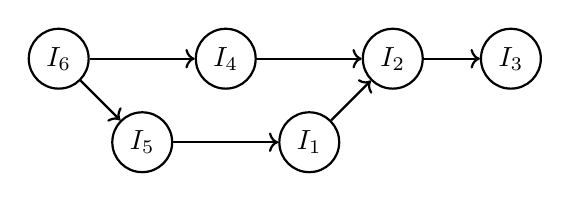
\begin{tikzpicture}[node distance={15mm}, thick, main/.style = {draw, circle}] 
\node[main] (6) {$I_6$}; 
\node[main] (5) [below right of=6] {$I_5$}; 
\node[main] (4) [above right of=5] {$I_4$};
\node[main] (1) [below right of=4] {$I_1$}; 
\node[main] (2) [above right of=1] {$I_2$}; 
\node[main] (3) [right of=2] {$I_3$}; 
\draw[->] (6) -- (5); 
\draw[->] (5) -- (1);
\draw[->] (1) -- (2);
\draw[->] (2) -- (3);
\draw[->] (6) -- (4);
\draw[->] (4) -- (2);
\end{tikzpicture}
\end{center}
Note that, in this example, the directed graph of $\mapsto$ is not linear even though the graphs of each $\mapsto_s$ are. This reflects the fact that while this example is locally sequential, it is not globally sequential. 

Before characterizing this distinction in this formalization another key definition is needed. Given any measurement chain we can define another new relation by taking the reflexive transitive closure\footnote{Roughly, the reflexive transitive closure of a relation $Q$ is this relation plus $aQa$ for every $a$ and $aQb$ for every $a$ and $b$ where for some $c$ we have $aQc\land cQb$. This last step is done repeatedly until convergence. Concretely, $Q^\text{RTC}$ is the smallest extension of $Q$ which is transitive and reflexive. Namely, it is the intersection of all of the extensions of $Q$ which are reflexive and transitive.} of $\mapsto$ (notated $\mapsto^\text{RTC}$). According to this new relation $i\mapsto^\text{RTC}j$ just in case either $i=j$ or some sequence of systems and interactions connect $i$ to $j$ via their inputs and outputs. 

In many cases, it will be natural to demand that each interaction $i$ has $i\mapsto^\text{RTC} j$ for some record keeping interaction $j$. Otherwise, it seems like $i$ is irrelevant to the end state of the experiment. In our running example, $I_3$ is the only record keeping interaction and moreover every interaction $i$ has $i\mapsto^\text{RTC} I_3$.

We can now characterize strongly, globally, and locally sequential measurement chains in this formalization. 

A measurement chain is globally sequential just in case  $\mapsto^\text{RTC}$ is a total ordering. Our running example is not globally sequential, but would be if we dropped interaction $I_4$.

A measurement chain is strongly sequential just in case it is globally sequential, all its interactions are pair-wise (with $\vert S_i\vert=2$) and moreover $\vert S\vert=\vert I\vert+1$. This allows us to define a total ordering over $S$.

By contrast, in this formalization, a measurement chain is locally sequential when for each $s\in S$ we have that $\mapsto^\text{RTC}_s$ is a total ordering along with a compatibility constraint. Specifically, the set of relations $\{\mapsto_s\}$ is compatible if and only if $\mapsto^\text{RTC}$ is at least a partial ordering. Note that our running example is locally sequential. 

But what exactly is this compatibility constraint doing? In general, for any relation $Q$ we have that $Q^\text{RTC}$ is a partial order if and only if $Q$ is acyclic: there is no $N>1$ and no sequence $a_1,\dots, a_N$ such that $a_n Q a_{n+1}$ and $a_N=a_1$. Thus, explicitly, the compatibility criteria here for $\{\mapsto_s\}_{s\in S}$ is just that $\mapsto$ is acyclic. The measurement chain having $\mapsto$ acyclic means that there are no circular dependencies.

How could this have failed for a locally sequential measurement chain? Consider Fig.~\ref{FigChain2}, with each $\mapsto_s$ being linear but having different orientations, some right-to-left and some left-to-right. In such a case $\mapsto$ would have been cyclic. Compatibility ensures all of our systems agree about what ``later'' means.

Given this characterization, if we are to move away from locally sequential measurement chains, we need to consider $\mapsto_s$ which do not lead to $\mapsto^\text{RTC}_s$ being a total ordering. As I will now discuss, it is useful to characterize measurement chains which are not locally-sequential into two types depending on whether $\mapsto^\text{RTC}_s$ is partial ordering or not.

Let us then define a measurement chain to be \textit{locally partially ordered} when for each $s\in S$ we have that $\mapsto^\text{RTC}_s$ is a partial ordering and moreover the $\mapsto_s$ relations are compatible such that $\mapsto^\text{RTC}$ is also a partial ordering. Demanding that each $\mapsto^\text{RTC}_s$ is a partial ordering is equivalent to demanding that each $\mapsto_s$ is acyclic. Thus an alternate name for such measurement chains might be to call them \textit{locally acyclic} measurement chains. In the following subsection we will see a QFT-based example of a locally acyclic measurement chain which is not locally sequential.

By contrast, let us then define a measurement chain to be \textit{locally cyclic} when for at least one $s\in S$ we have $\mapsto_s$ being cyclic. From this it follows that neither $\mapsto^\text{RTC}_s$ nor $\mapsto^\text{RTC}$ are partial orders. In the following subsection we will see a QFT-based example of a cyclic measurement chain.

\subsection{Two QFT-based Examples}\label{Appendix1.3}
Let us now apply this formalization to a QFT experiment. In particular, let us consider an entanglement harvesting experiment. Roughly, in such an experiment (e.g., ~\cite{Valentini1991, Reznik2003, Pozas-Kerstjens:2015,Menicucci, Terno2016, Cosmo, Henderson2018,Ruep2021}) two initially uncorrelated probe systems interact locally with a quantum field in such a way that they do not have time to signal to each other. Despite this, these two probes become entangled because there was already entanglement present between the two space-like separated regions they interacted with. The benefit of such an experiment is that the entanglement in the field has been transferred into more accessible systems, both physically and mathematically. The final entanglement of these probes is a witness to the initial entanglement in the field.

Consider the following experiment: A quantum field, $\phi$, comes to a cold global thermal equilibrium by some process in the past of our experiment (in region $R_0$ in Fig.\ref{FigEntHarv}). Following this entanglement is harvested from this field by local interactions with two initially uncorrelated probe systems, let's call them $\text{Probe}$ 1 and $\text{Probe}$ 2. Specifically, $\text{Probe}$ 1 undergoes local interactions with $\phi$ in regions $R_1$, $R_2$, and $R_3$. $\text{Probe}$ 2 interacts with $\phi$ in region $R_4$. Each of these probes later interact with some measurement device $M_1$ and $M_2$ in regions $R_5$ and $R_6$ respectively. The correlation between the outputs of these measurement devices confirms that the probes were entangled after their interaction with $\phi$. Our experiment might then investigate how the amount of entangle harvested depends on various factors: the initial temperature of $\phi$, the strengths of various interactions, etc. 

\begin{figure}
\includegraphics[width=0.45\textwidth]{Figures/EntHarvDiagram.pdf}
\caption{The space-time regions involved in the entanglement harvesting experiment formalized in Appendix \ref{Appendix1}.}\label{FigEntHarv}
\end{figure}

Let us now design a measurement chain to help us guide us in modeling this experiment. Firstly, regarding the thermalization of the field, $\phi$, we may reasonably leave this process out of our modeling and just assume that $\phi$ starts in a global thermal state. Next we must consider how to model the probe systems. Roughly, our options are either to model them as QFTs (e.g., in the FV framework) or as non-relativistic quantum systems (e.g., as a UDW detector) localized around some trajectory. See Sec.~\ref{StateOfTheArt} for details.

Given the spacetime relations between $R_1$, $R_2$ and $R_3$ we cannot model Probe 1 as a non-relativistic system localized around some trajectory. No time-like trajectory can get us from $R_1$ to $R_3$. Thus, we are forced to model Probe 1 as a QFT, let's call it $\psi$. Regarding Probe 2, no such barrier exists. Let us suppose that we can model this probe well as a UDW detector. 

The interactions in $R_5$ and $R_6$ are with measurement devices $M_1$ and $M_2$. It is doubtful we can model these systems or the measurement processes within QFT. Thus, between $R_1$-$R_3$ and $R_5$ we will need to switch to describing $\psi$ within non-relativistic quantum theory. These measurements can then both be handled well within our already established non-relativistic quantum measurement theory. 

Let's transfer the above considerations into a formalized measurement chain. We have five systems: $\phi$ the field the entanglement is being harvested from, $\psi$ a probe field, $\text{UDW}$ a Unruh DeWitt detector, two measurement apparatuses, $M_1$ and $M_2$. Three theories are relevant to this measurement chain: $T_1$, quantum field theory, $T_2$, non-relativistic quantum theory, and $T_3$ being classical theory. These systems undergo six interactions as indicated by the following table:
\[\begin{array}{cccccccc}
H(s,i) & \vert & I_1 & I_2 & I_3 & I_4 & I_5 & I_6\\
\phi & \vert & T_1 & T_1 & T_1 & T_1 & \emptyset & \emptyset\\
\psi & \vert & T_1 & T_1 & T_1 & \emptyset & T_2 & \emptyset\\
\text{UDW} & \vert & \emptyset & \emptyset & \emptyset & T_2 & \emptyset & T_2\\
M_1 & \vert & \emptyset & \emptyset & \emptyset & \emptyset & T_2 & \emptyset\\
M_2 & \vert & \emptyset & \emptyset & \emptyset & \emptyset & \emptyset & T_2\\
\end{array}\]
Already we can see that our measurement chain involves a diagonal cut in $I_4$ between $\phi$ and our $\text{UDW}$ detector. This is a diagonal QFT-cut because a QFT is coupled to a non-QFT.

Next we need to specify $\mapsto_s$. How do these spacetime relations in Fig. \ref{FigEntHarv} determine the relations $\mapsto_s$? We can understand an interaction's ``outputs'' in the above formalization as meaning any future oriented time-like or light-like trajectories leaving the spacetime region associated with an interaction. We can similarly understand an interaction's ``inputs''. Thus, in this context\footnote{Applied to other problems, one may want to add an extra condition here that these time-like or light-like trajectories are not allowed to travel through other interaction regions. If all paths from $R_A$ to $R_C$ lead through $R_B$, it makes more sense to understand $I_A$ as having no output into $I_C$. Rather, we can then understand $I_A$ to output into $I_B$ which then outputs into $I_C$.} we can define $i\mapsto_s j$ if and only if $s@i$ and $s@j$ and there is future directed time-like or light-like curve beginning in $R_i$ and ending in $R_j$. Taking $\mapsto_s$ to be determined in this way, we have:
\[\begin{array}{ccl}
S & \vert & \text{Directed Graph of }\mapsto_s\text{ over }I_s\\
\phi & \vert & I_1\mapsto_\phi I_2\mapsto_\phi I_3, \quad I_4\\
\psi & \vert & (\text{See Below})\\
\text{UDW} & \vert & I_4\mapsto_\text{UDW} I_6\\
M_1 & \vert & I_5\\
M_2 & \vert & I_6\\
\end{array}\]
The relation $\mapsto_\psi$ in this case is:
\begin{center}
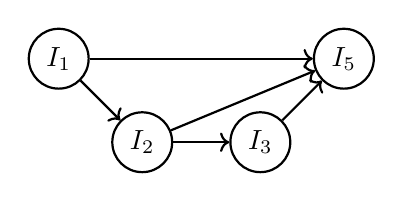
\begin{tikzpicture}[node distance={15mm}, thick, main/.style = {draw, circle}] 
\node[main] (1) {$I_1$}; 
\node[main] (2) [below right of=1] {$I_2$}; 
\node[main] (3) [right of=2] {$I_3$};
\node[main] (5) [above right of=3] {$I_5$}; 
\draw[->] (1) -- (2); 
\draw[->] (2) -- (3);
\draw[->] (1) -- (5);
\draw[->] (2) -- (5);
\draw[->] (3) -- (5);
\end{tikzpicture}
\end{center}
The first thing to notice here is that the directed graph for $\mapsto_\phi$ is composed of two disjoint subgraphs. It follows from this that $\mapsto_\phi^\text{RTC}$ is not a total order and therefore this measurement chain is not locally sequential. Next, notice that one interaction may have multiple outputs for a single system: $I_1\mapsto_\psi I_2$ and $I_1\mapsto_\psi I_5$. This has not occurred in any previous example. Secondly, notice that it is not the case that $I_1\mapsto_\psi I_3$ even though $I_1\mapsto_\psi I_2$ and $I_2\mapsto_\psi I_3$. That is, $\mapsto_\psi$ is not transitive. The relation, $\mapsto_\psi^\text{RTC}$, however is transitive but importantly can't be interpreted straightforwardly in terms of spacetime regions.

The directed graph for $\mapsto$ is:
\begin{center}
\begin{tikzpicture}[node distance={15mm}, thick, main/.style = {draw, circle}] 
\node[main] (1) {$I_1$}; 
\node[main] (2) [below right of=1] {$I_2$}; 
\node[main] (3) [right of=2] {$I_3$};
\node[main] (6) [above of=5] {$I_6$};
\node[main] (5) [above right of=3] {$I_5$}; 
\node[main] (4) [left of=6] {$I_4$};
\draw[->] (1) -- (2); 
\draw[->] (2) -- (3);
\draw[->] (1) -- (5);
\draw[->] (2) -- (5);
\draw[->] (3) -- (5);
\draw[->] (4) -- (6);
\end{tikzpicture}
\end{center}
Notice that the directed graph for $\mapsto$ is composed of two disjoint subgraphs. This has not happened before in any previous examples. The fact that this happens here actually reflects a central consideration in this entanglement harvesting experiment. For the entanglement between $\psi$ and $\text{UDW}$ to be cleanly associated with space-like entanglement in the field $\phi$ their interactions and measurements need to be isolated from each other.

The last thing we need to do to specify our measurement chain is to define the $Z$ function. $Z$ here is given by:
\[\begin{array}{cccccccc}
Z(s,i) & \vert & I_1 & I_2 & I_3 & I_4 & I_5 & I_6\\
\phi & \vert & X & X & X & X & \emptyset & \emptyset\\
\psi & \vert & X & X & X & \emptyset & X & \emptyset\\
\text{UDW} & \vert & \emptyset & \emptyset & \emptyset & X & \emptyset & X\\
M_1 & \vert & \emptyset & \emptyset & \emptyset & \emptyset & T_3 & \emptyset\\
M_2 & \vert & \emptyset & \emptyset & \emptyset & \emptyset & \emptyset & T_3\\
\end{array}\]
The only interactions which are directly relevant to the end of the experiment are the measurements at $I_5$ and $I_6$. As the above table indicates, the states of $M_1$ and $M_2$ following these interactions will be modeled in $T_3$, i.e., classically.

The vertical cuts in this measurement chain are as follows. Between $I_1$-$I_3$ and $I_5$ we have a vertical cut on $\psi$ from $T_1$ to $T_2$. That is, after $\psi$ is done probing $\phi$ we need to switch to modeling it as a non-relativistic quantum system. There are many options available as to how one might do this, see Sec.~\ref{StateOfTheArt}. In any case, this is a vertical QFT-cut. There are also two vertical Heisenberg cuts on $M_1$ and $M_2$ following the interactions $I_5$ and $I_6$ respectively.  

We have thus formalized a non-locally-sequential measurement chain. This measurement chain was, however, acyclic. That is, $\mapsto$ is acyclic such that $\mapsto^\text{RTC}$ is a partial order. As I suggested in the previous subsection, this will not always be the case. Consider for instance, the spacetime regions shown in Fig. \ref{FigCyclic}. Consider a field $f$ which undergoes interactions $i$ and $j$ localized in these regions. In accordance with our above discussion we would have $i\mapsto_f j$ and $j\mapsto_f i$. This is because a part of $R_i$ is in the future of $R_j$ and likewise part of $R_j$ is in the future of $R_i$. The formalization presented in the previous subsection is flexible enough to handle such examples. 

\begin{figure}
\includegraphics[width=0.45\textwidth]{Figures/CyclicDiagram.pdf}
\caption{Spacetime regions which would lead to a cyclic measurement chain. Regions $R_i$ and $R_j$ are both before and after each other in a sense.}\label{FigCyclic}
\end{figure}

\subsection{Proving the Necessity of Cuts} 
Having so formalized modelings of measurement chains, let's now prove the claim in the main paper regarding under what conditions cuts are required. In particular, let us now prove the following claim: If one part of the experiment must be modeled some way and another later part must not be modeled in this way then somewhere in between these we need to make a certain kind of cut. 

Formalizing this claim we understand the first part of the experiment as referring to a system $s$ at one of its interactions $i$ with $s@i$. The second part of the experiment mentioned above could is understood as a system $t$ \textit{either at or after} one of its interactions $j$ with $t@j$. In the first case we will be concerned with $H(t,j)$ and in the second case $Z(t,j)$. We understand the ``must (must not) be modeled in some way'' here as specifying some subset of our theories $V\subset T$ and fixing $H(s,i)\in V$ and $H(t,j)\notin V$ (or alternatively $Z(t,j)\notin V$). We understand the claim that the second part of the experiment is ``later'' as\footnote{Note that given the discussion in the previous subsection, one must be careful when trying to interpret $\mapsto^\text{RTC}$ in terms of spacetime relations.}. Finally, we can understand the ``the certain kind of cut'' here to mean either a vertical or a diagonal $V$ cut.%We might have $i\mapsto^\text{RTC}j$ while $R_i$ and $R_j$ are space-like separated. Despite this there is still a clear sense in which $i\mapsto^\text{RTC}j$ means $j$ is later than $i$.} $i\mapsto^\text{RTC}j$. The claim that a cut happens ``in between'' can be understood as meaning between according to $\mapsto^\text{RTC}$. That is, at some $k$ with \mbox{$i\mapsto^\text{RTC} k \mapsto^\text{RTC} j$

Thus the formalized claim is as follows. Suppose we are given any modeling of a measurement chain and are given some $s_0,t_0\in S$ and $i_0,j_0\in I$ with $s_0@i_0$ and $t_0@j_0$ and \mbox{$i_0 \mapsto^\text{RTC}j_0$}. Suppose further that $H(s_0,i_0)\in V$ and either $H(t_0,j_0)\notin V$ or if \mbox{$Z(t_0,j_0)\neq X$} then \mbox{$Z(t_0,j_0)\notin V$}. In such cases, there must be some interaction $k$ with \mbox{$i_0\mapsto^\text{RTC} k \mapsto^\text{RTC} j_0$} where either a diagonal or vertical $V$ cut happens.

Proof: Suppose for contradiction that no such cut occurs. I will show that this implies that $H(t_0,j_0)\in V$ and if $Z(t_0,j_0)\neq X$ then $Z(t_0,j_0)\notin V$. This would be in explicit contradiction with our above assumptions.

First, note that no vertical $V$ cuts implies that for all $s\in S$ and $i,j\in I_s$ with $i\mapsto_s j$ we have \mbox{$H(s,i)\in V\implies H(s,j)\in V$}. Similarly, if $Z(s,i)\neq X$ then \mbox{$H(s,i)\in V\implies Z(s,i)\in V$}. Similarly, no diagonal $V$ cuts implies that for all $i\in I$ and $s,t\in S_i$ we have \mbox{$H(s,i)\in V\implies H(t,i)\in V$}. As I will now show, our desired result follows from a series of applications of these three implications.

To see this, begin by noting that $i_0\mapsto^\text{RTC}j_0$ means that there exists some sequence of interactions $k_1,\dots,k_N\in I$ and some corresponding sequence of systems $x_0,\dots,x_N\in S$ with, 
\begin{align}\label{ProofEq1}
i\mapsto_{x_0}k_1\mapsto_{x_1}\dots\mapsto_{x_{N-1}}k_N\mapsto_{x_N} j.    
\end{align}
This follows from the definition of $\mapsto^\text{RTC}$ as the reflexive transitive closure of $\mapsto$ and the definition of $\mapsto$ in terms of $\mapsto_s$. For the above sequence to make sense it is required that $k_n\in I_{x_n}\cap I_{x_{n-1}}$ That is, the interaction $k_n$ must involve both $x_n$ and $x_{n-1}$. 

We can decompose any such sequence into a series of ``runs'' where $x_n=\dots=x_{n+m-1}=y$ for some $m>0$ and some fixed $y\in S$. Such runs make repeated use of some $\mapsto_{y}$ as,
\begin{align}
k_n\mapsto_{y}k_{n+1} \mapsto_{y}\dots\mapsto_{y}k_{n+m}. 
\end{align}
Note that because no vertical $V$ cuts are allowed we have \mbox{$H(y,k_n)\in V\implies H(y,k_{n+1})\in V$}. Applying this logic repeatedly we ultimately have \mbox{$H(y,k_n)\in V\implies H(y,k_{n+m})\in V$}. Thus, moving along one of these $\mapsto_{y}$ runs cannot help us switch from theories in $V$ to theories in $T-V$.

What about at the interface between such runs? Namely, 
\begin{align}
\dots\mapsto_{y}k_{\ell-1}\mapsto_{y}k_\ell \mapsto_{z}k_{\ell+1}\mapsto_{z}\dots. 
\end{align}
with $y\neq z$ and  $y,z\in S_{k_\ell}$. Must we have \mbox{$H(z,k_{\ell+1})\in V$} if \mbox{$H(y,k_\ell)\in V$}? Yes, because we are not allowed diagonal cuts we must have \mbox{$H(y,k_n)\in V\implies H(z,k_n)\in V$}. Since $y$ and $z$ are both involved in the interaction $k_n$ they must both be modeled in $V$, anything otherwise would give rise to a diagonal $V$ cut. However, then by our above logic, without vertical cuts we have \mbox{$H(z,k_\ell)\in V \implies H(z,k_{\ell+1})\in V$}.

Thus, without allowing for vertical cuts or diagonal $V$ cuts, we ultimately have \mbox{$H(s,i)\in V \implies H(t,j)\in V$} and therefore $H(t,j)\in V$. If $Z(t,j)\neq X$ then we have further that $Z(t,j)\in V$ since no vertical $V$ cuts implies \mbox{$H(t,j)\in V \implies Z(t,j)\in V$}.

In order to avoid this conclusion we need to allow for vertical or diagonal $V$ cuts. In particular, the above proof shows that we must either take a vertical $V$-cut right at the end, or otherwise at some point in sequence, Eq. \eqref{ProofEq1} connection $i$ and $j$ either type of cut must happen.

\end{document}